\documentclass{beamer}
\usetheme[block=fill, subsectionpage=progressbar]{metropolis}

\usepackage{amsmath}
\usepackage[style=numeric]{biblatex}
\usepackage{url}
\usepackage{caption}

\addbibresource{references.bib}

\title{Modelling Baseball Exit Velocities with Extreme Value Theory}
\subtitle{MATH 589 Final Project}
\author{Jules Lanari-Collard}
\institute{McGill University}
\date{November 29, 2024}

\begin{document}
\frame{\titlepage}
\section{Introduction}

\begin{frame}{Why?}
\begin{itemize}
    \item Average MLB franchise is worth \$2.4 billion \cite{forbesValuations}.
    \item 2nd most popular sport in US \cite{gallupPoll}.
    \item Median projected payroll for 2025 is \$144 M - some teams projected for over \$270 M \cite{fgRosterResource}.
    \item Shohei Ohtani signed for \$700 M over 10 years (2024-2033).
    \item Franchises employ dedicated analytics teams to inform decisions and evaluate players.
\end{itemize}
\end{frame}

\begin{frame}[allowframebreaks]{Why Exit Velocity Matters}
    \begin{figure}
        \centering
        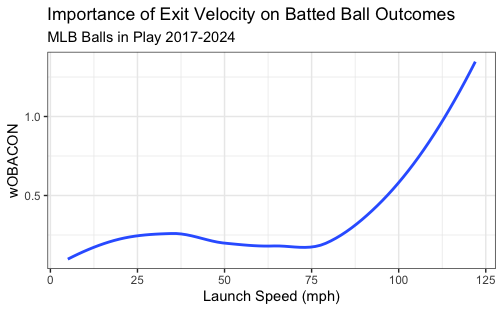
\includegraphics[width=0.85\linewidth]{plots/ev_woba.png}
    \end{figure}
    
    \begin{figure}
        \centering
        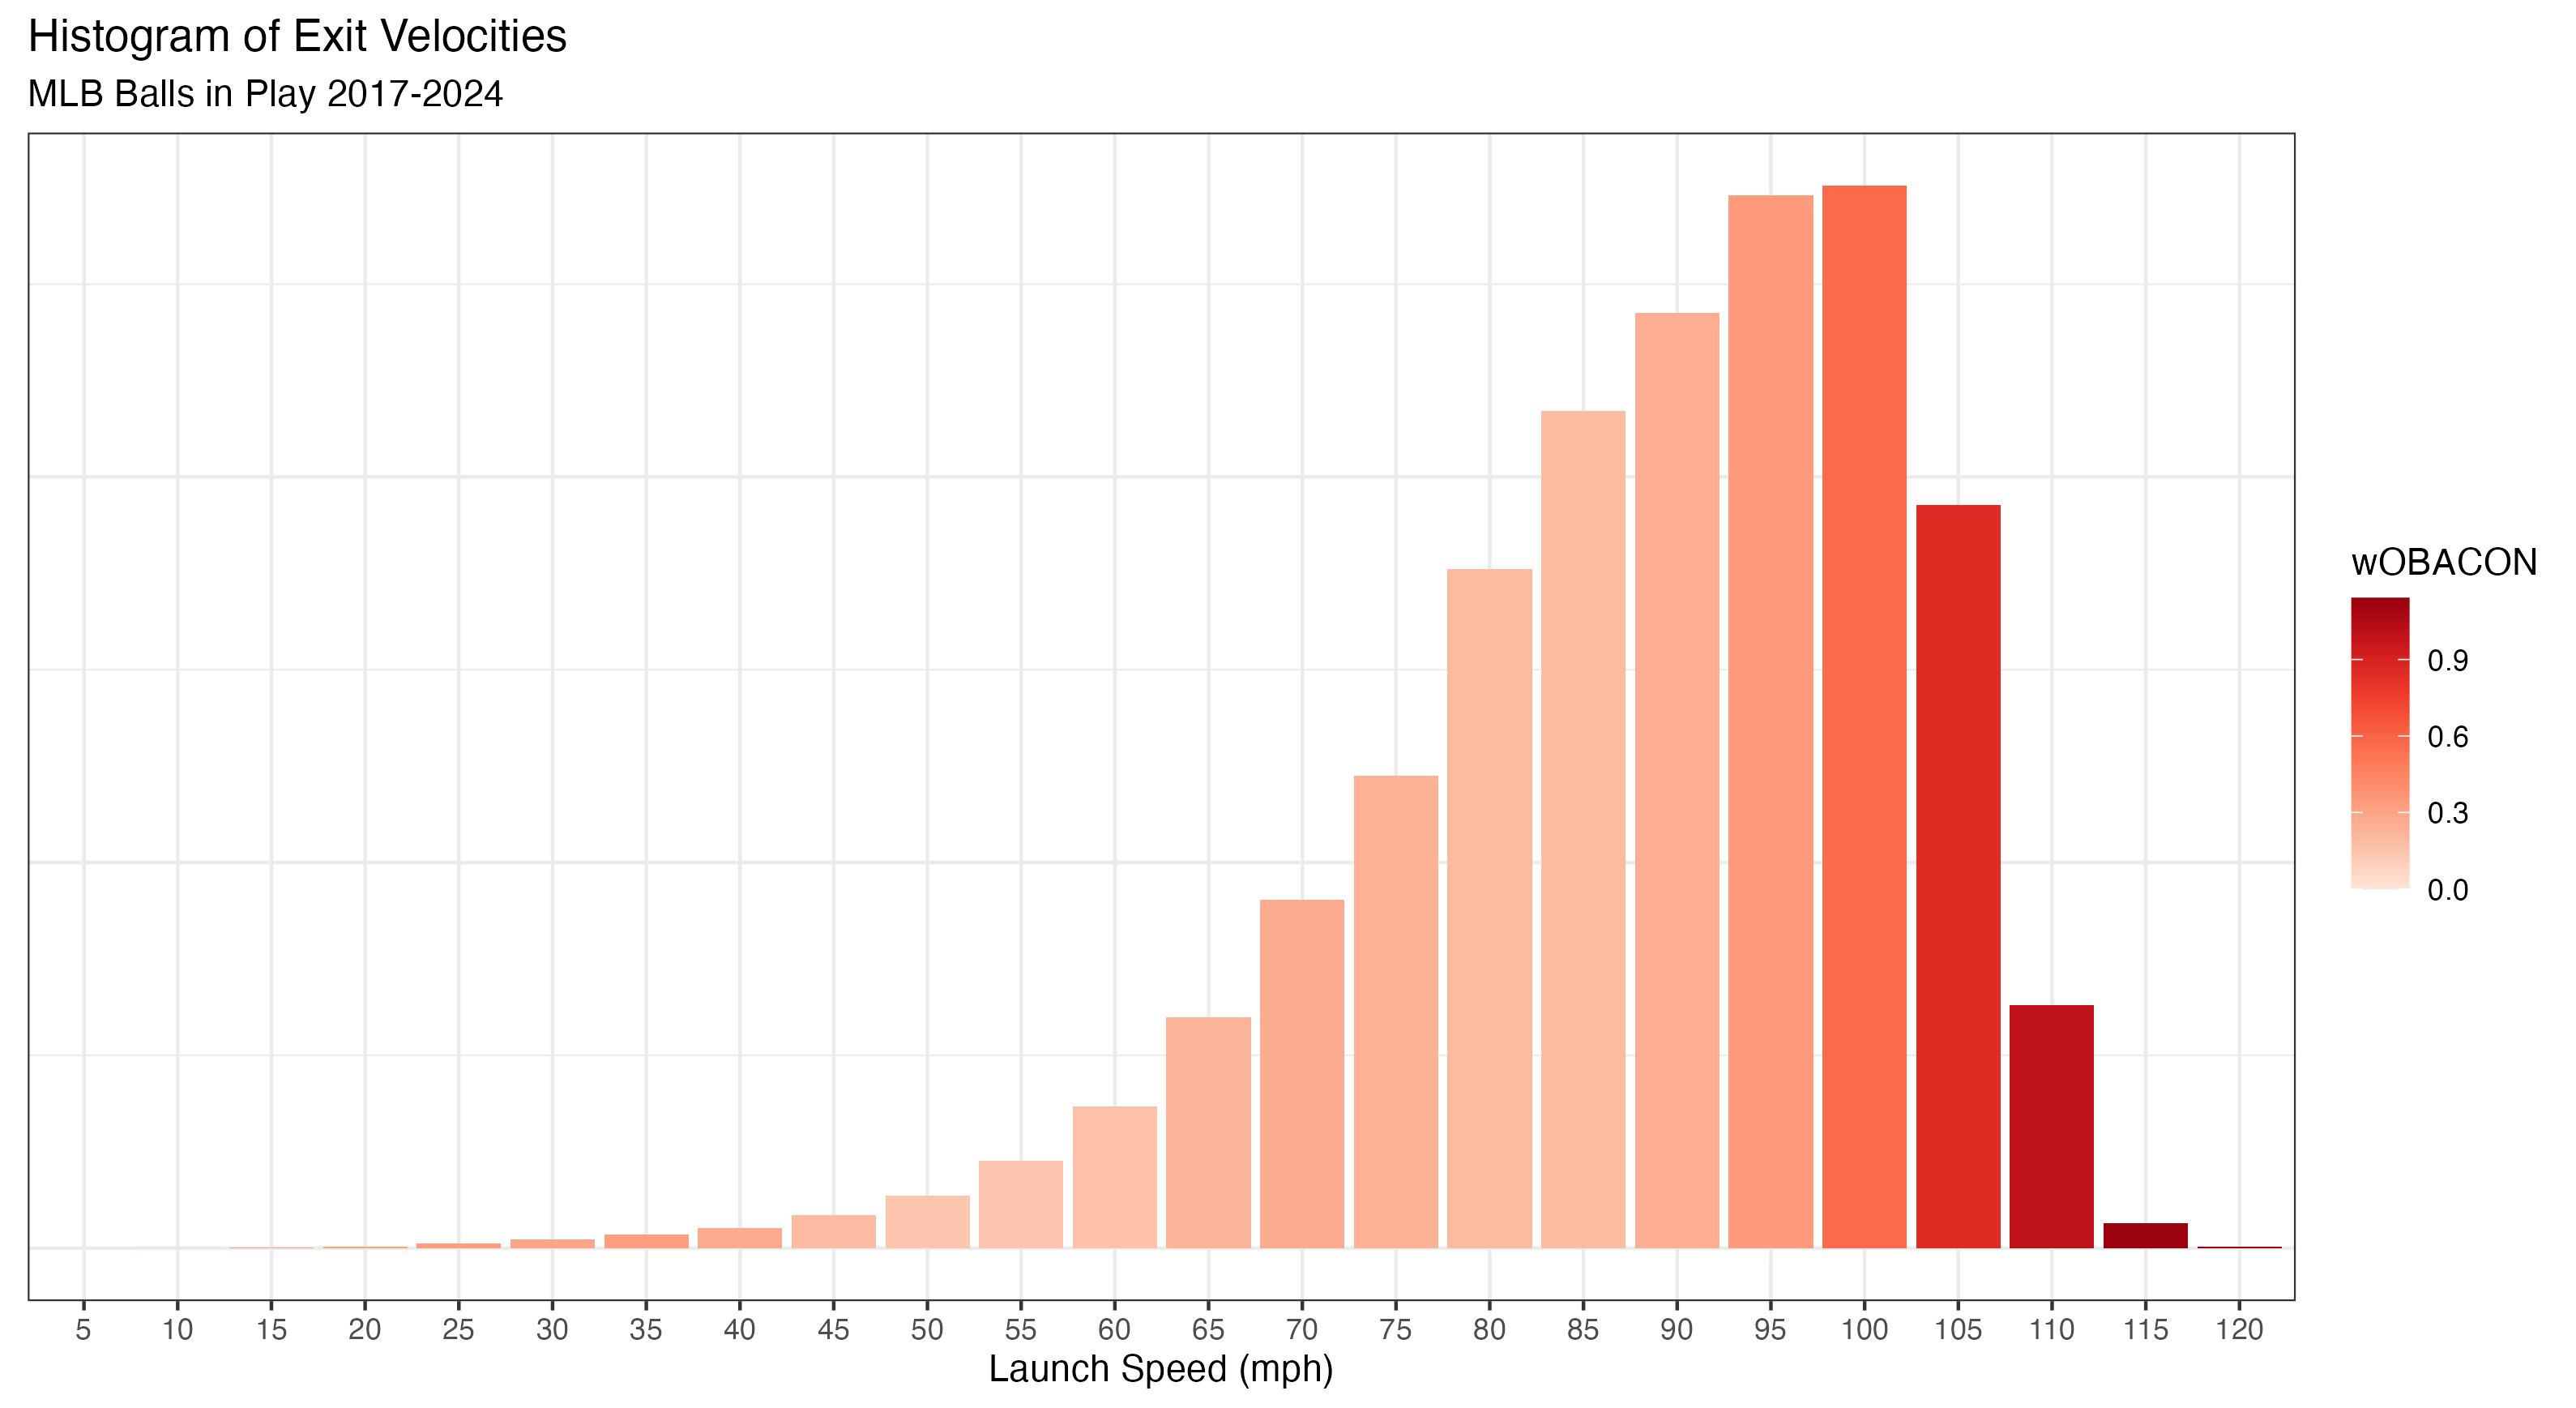
\includegraphics[width=0.85\linewidth]{plots/evHistogram.png}
    \end{figure}
\end{frame}

\begin{frame}{Player Distributions}
    Differing player types \& styles lead to different player-level EV distributions:
    \begin{figure}
        \centering
        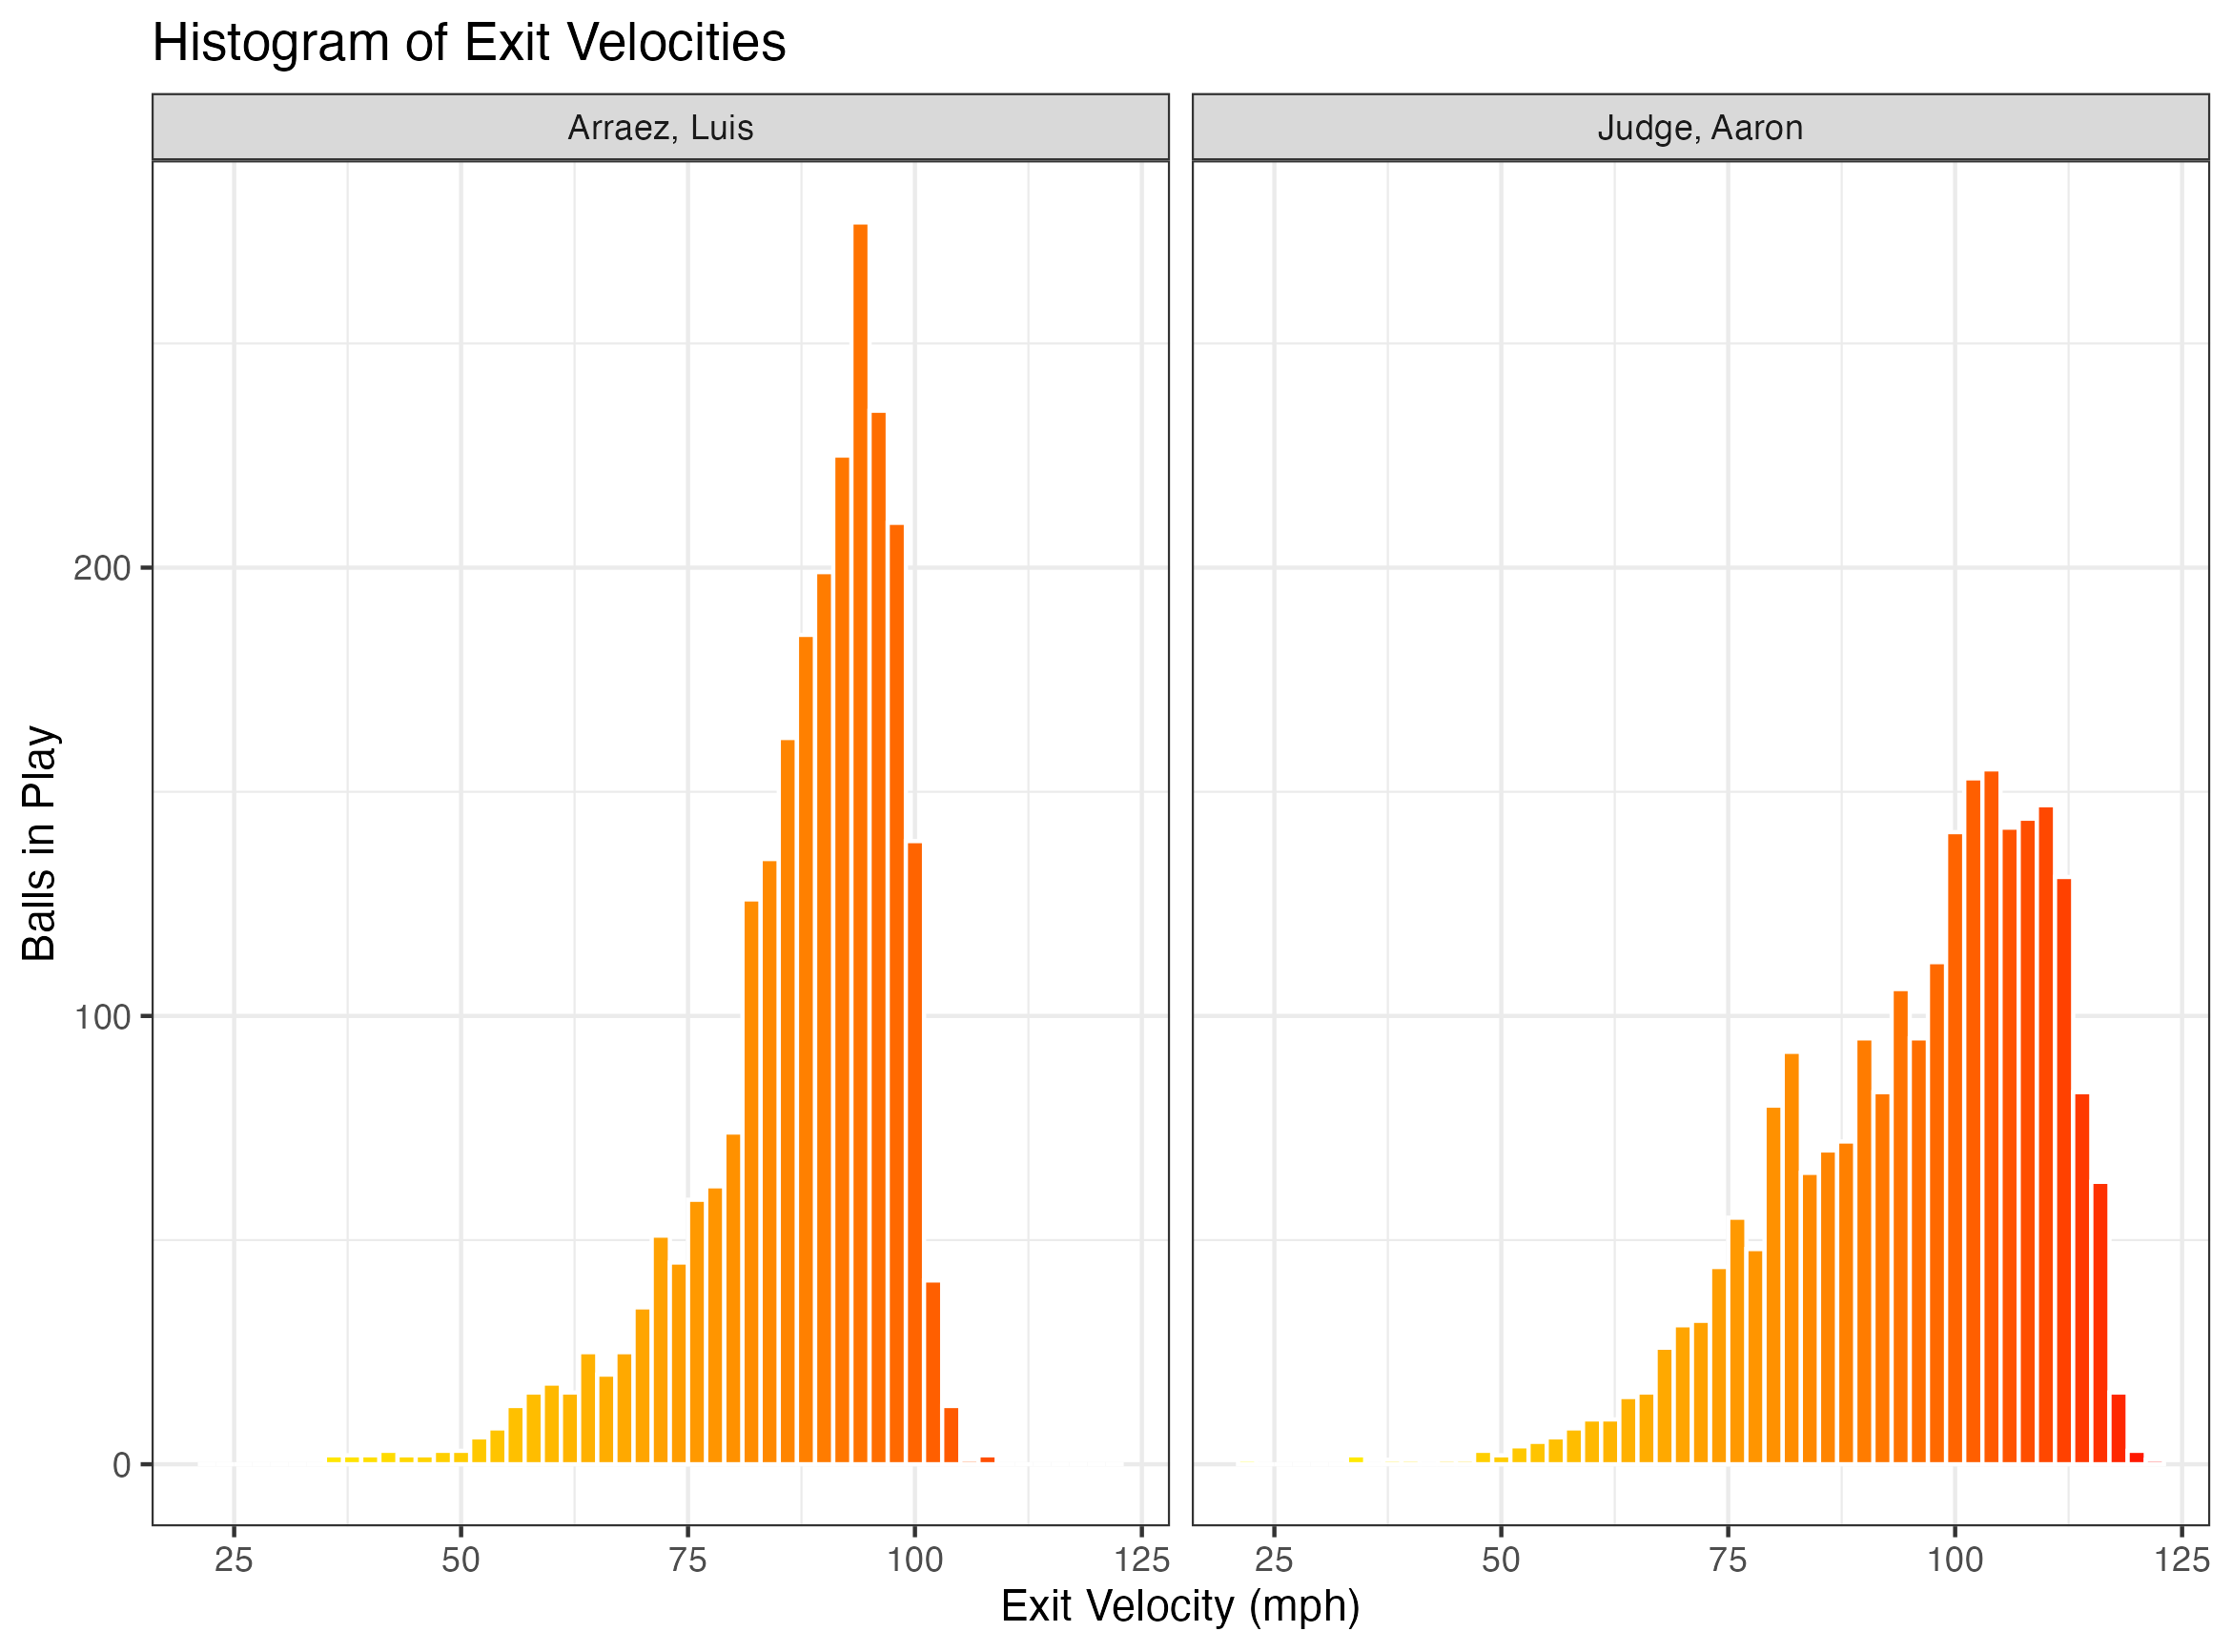
\includegraphics[width=0.85\linewidth]{plots/playerComparison.png}
    \end{figure}
\end{frame}

\begin{frame}{Existing Exit Velocity Metrics}
Most common/popular statistics to interpret EV data \cite{andrewsEV}:
\begin{itemize}
    \item Average EV
    \item Best Speed \cite{tangoBestSpeed}
    \begin{itemize}
        \item Average of top 50\% hardest-hit balls
    \end{itemize}
    \item EV Percentiles \cite{clemensEV}
    \begin{itemize}
        \item EV80, EV90 \& EV95
    \end{itemize}
    \item Maximum EV
    \item Hard-Hit \%
    \begin{itemize}
        \item \% of balls hit $>$95mph
    \end{itemize}
\end{itemize}
\end{frame}

\section{A New Approach}
\begin{frame}{Modelling EV}
    \begin{itemize}
        \item Distributions of EV vary by player
        \item We do not learn anything about a player's talent from their slowly-hit batted balls \cite{tangoBestSpeed}.
        \item Information lies in the upper quantiles of a player's EV distribution. 
    \end{itemize}
    Extreme Value Theory!
\end{frame}

\begin{frame}[allowframebreaks]{Block Maxima}
    Fitted GEV to each player's 10 BIP block-maxima:
    \begin{figure}
        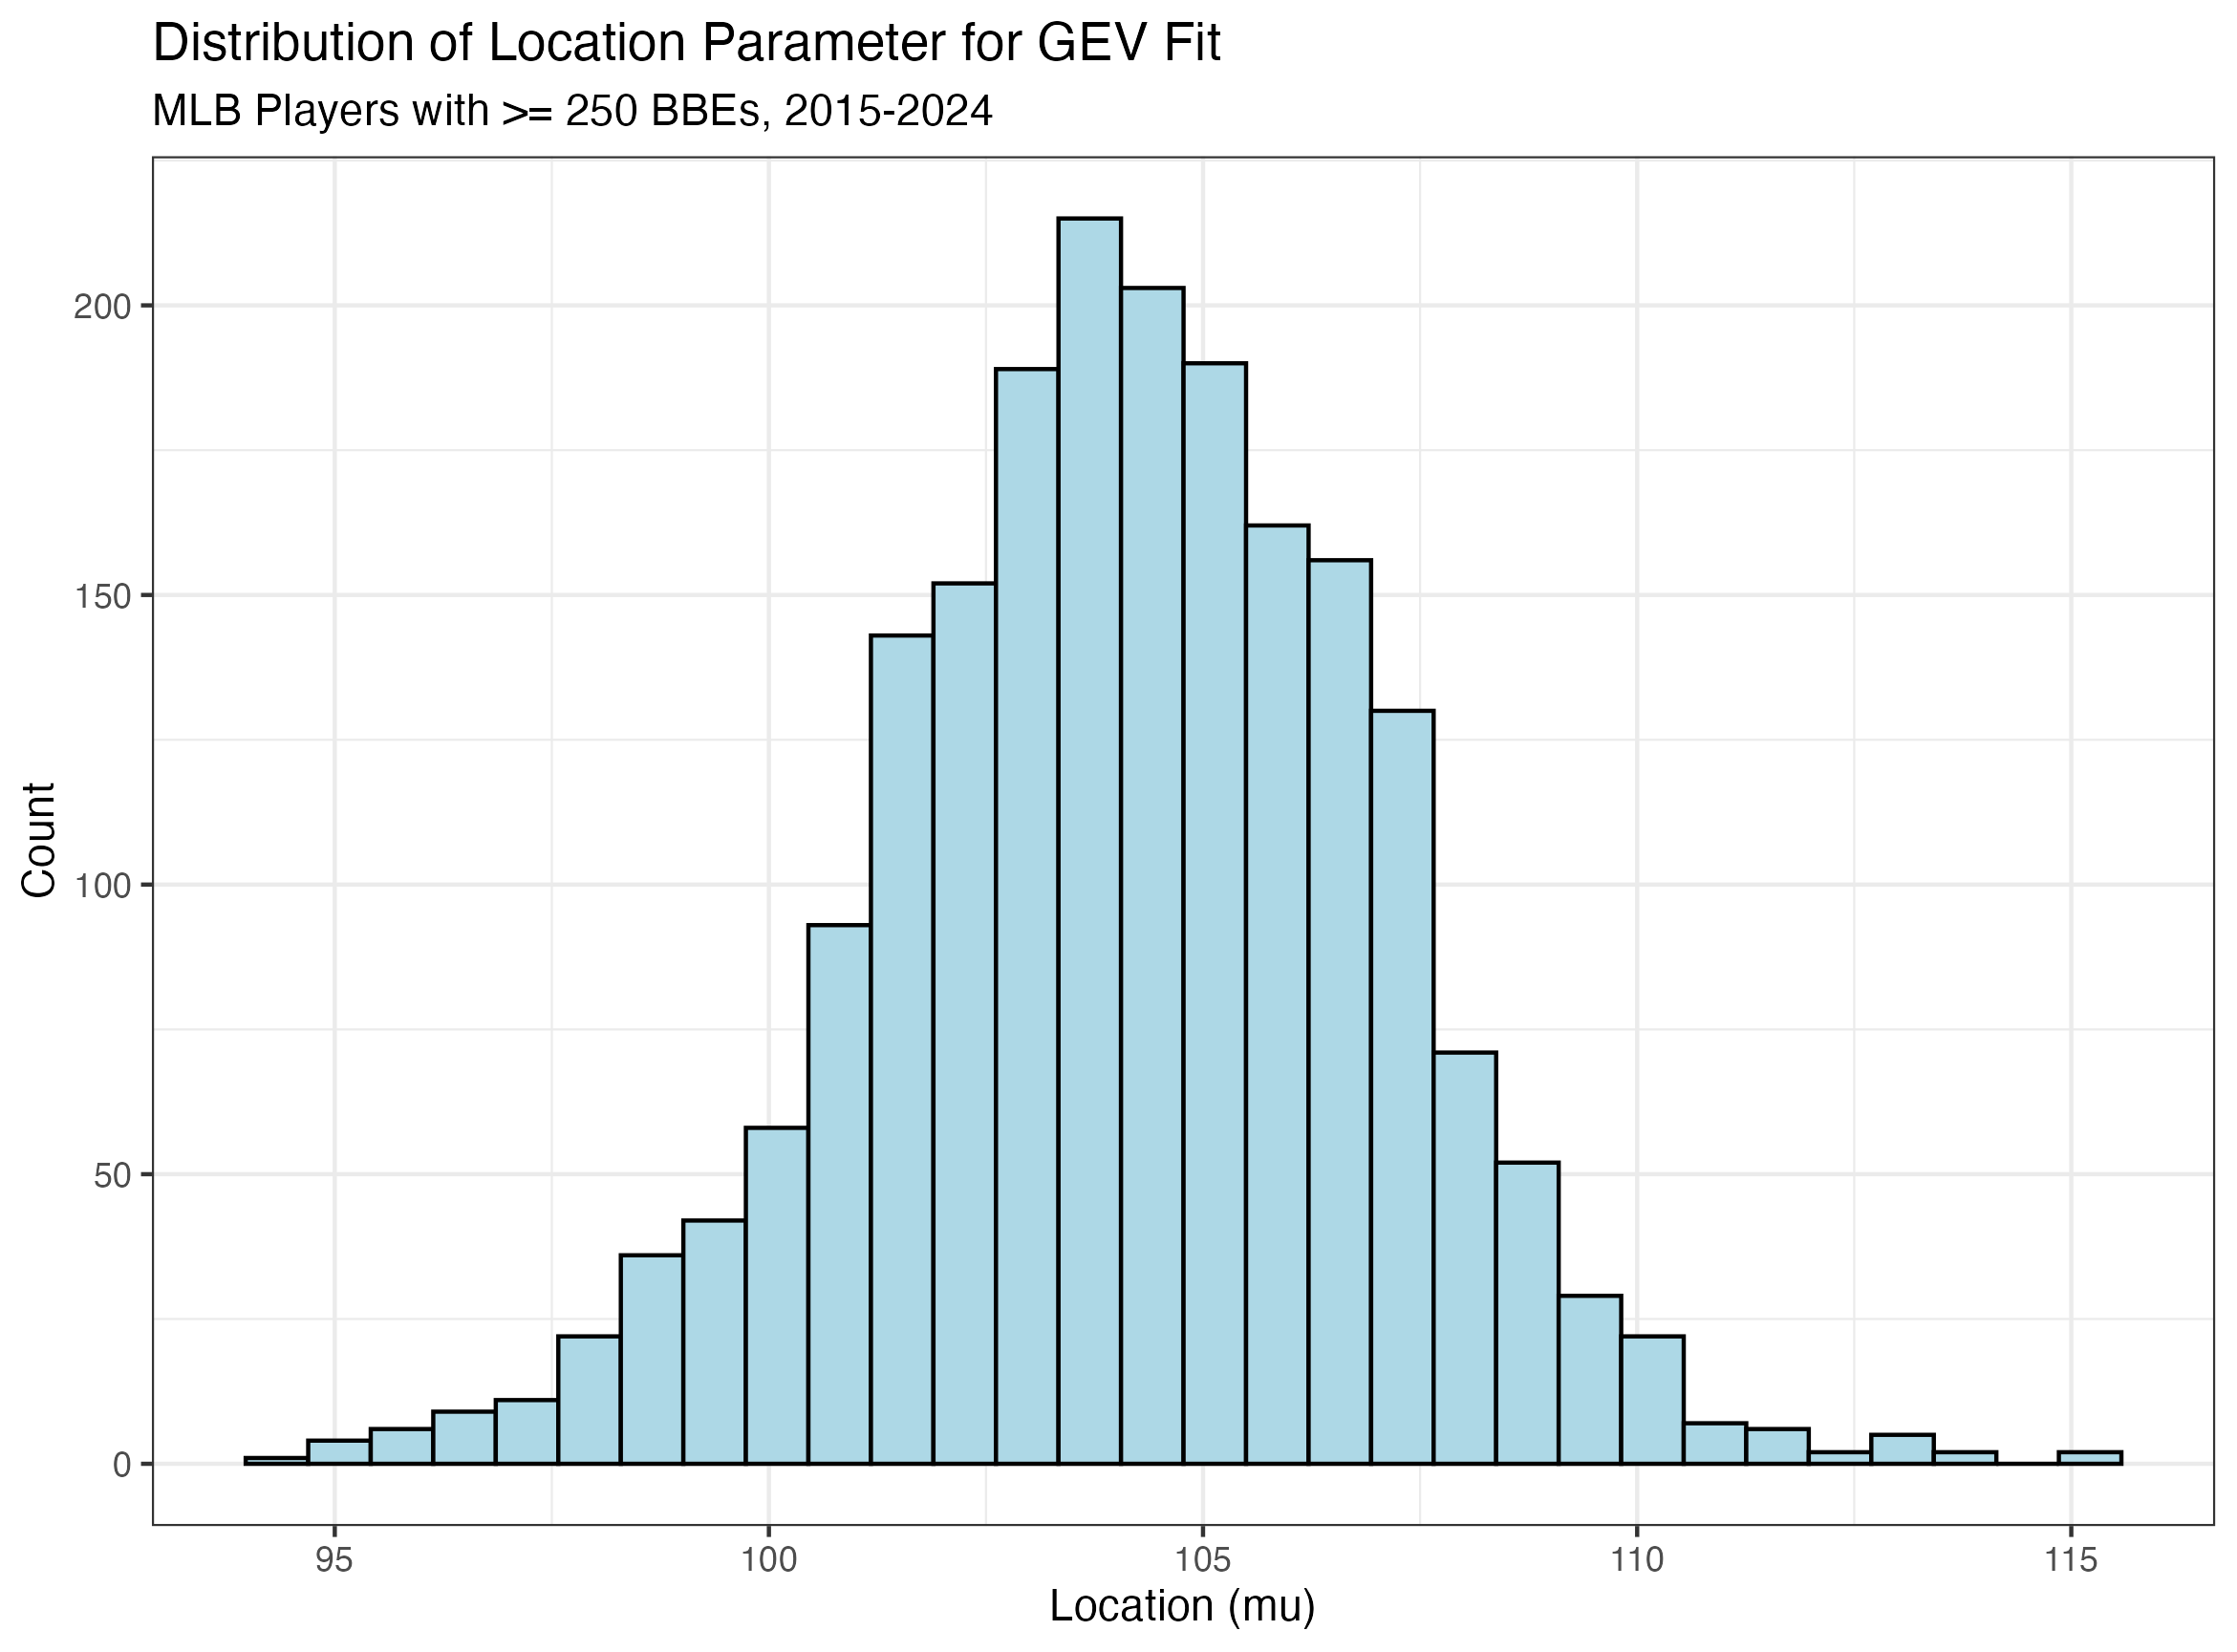
\includegraphics[width=0.49\linewidth]{plots/location.png}
        \hfill
        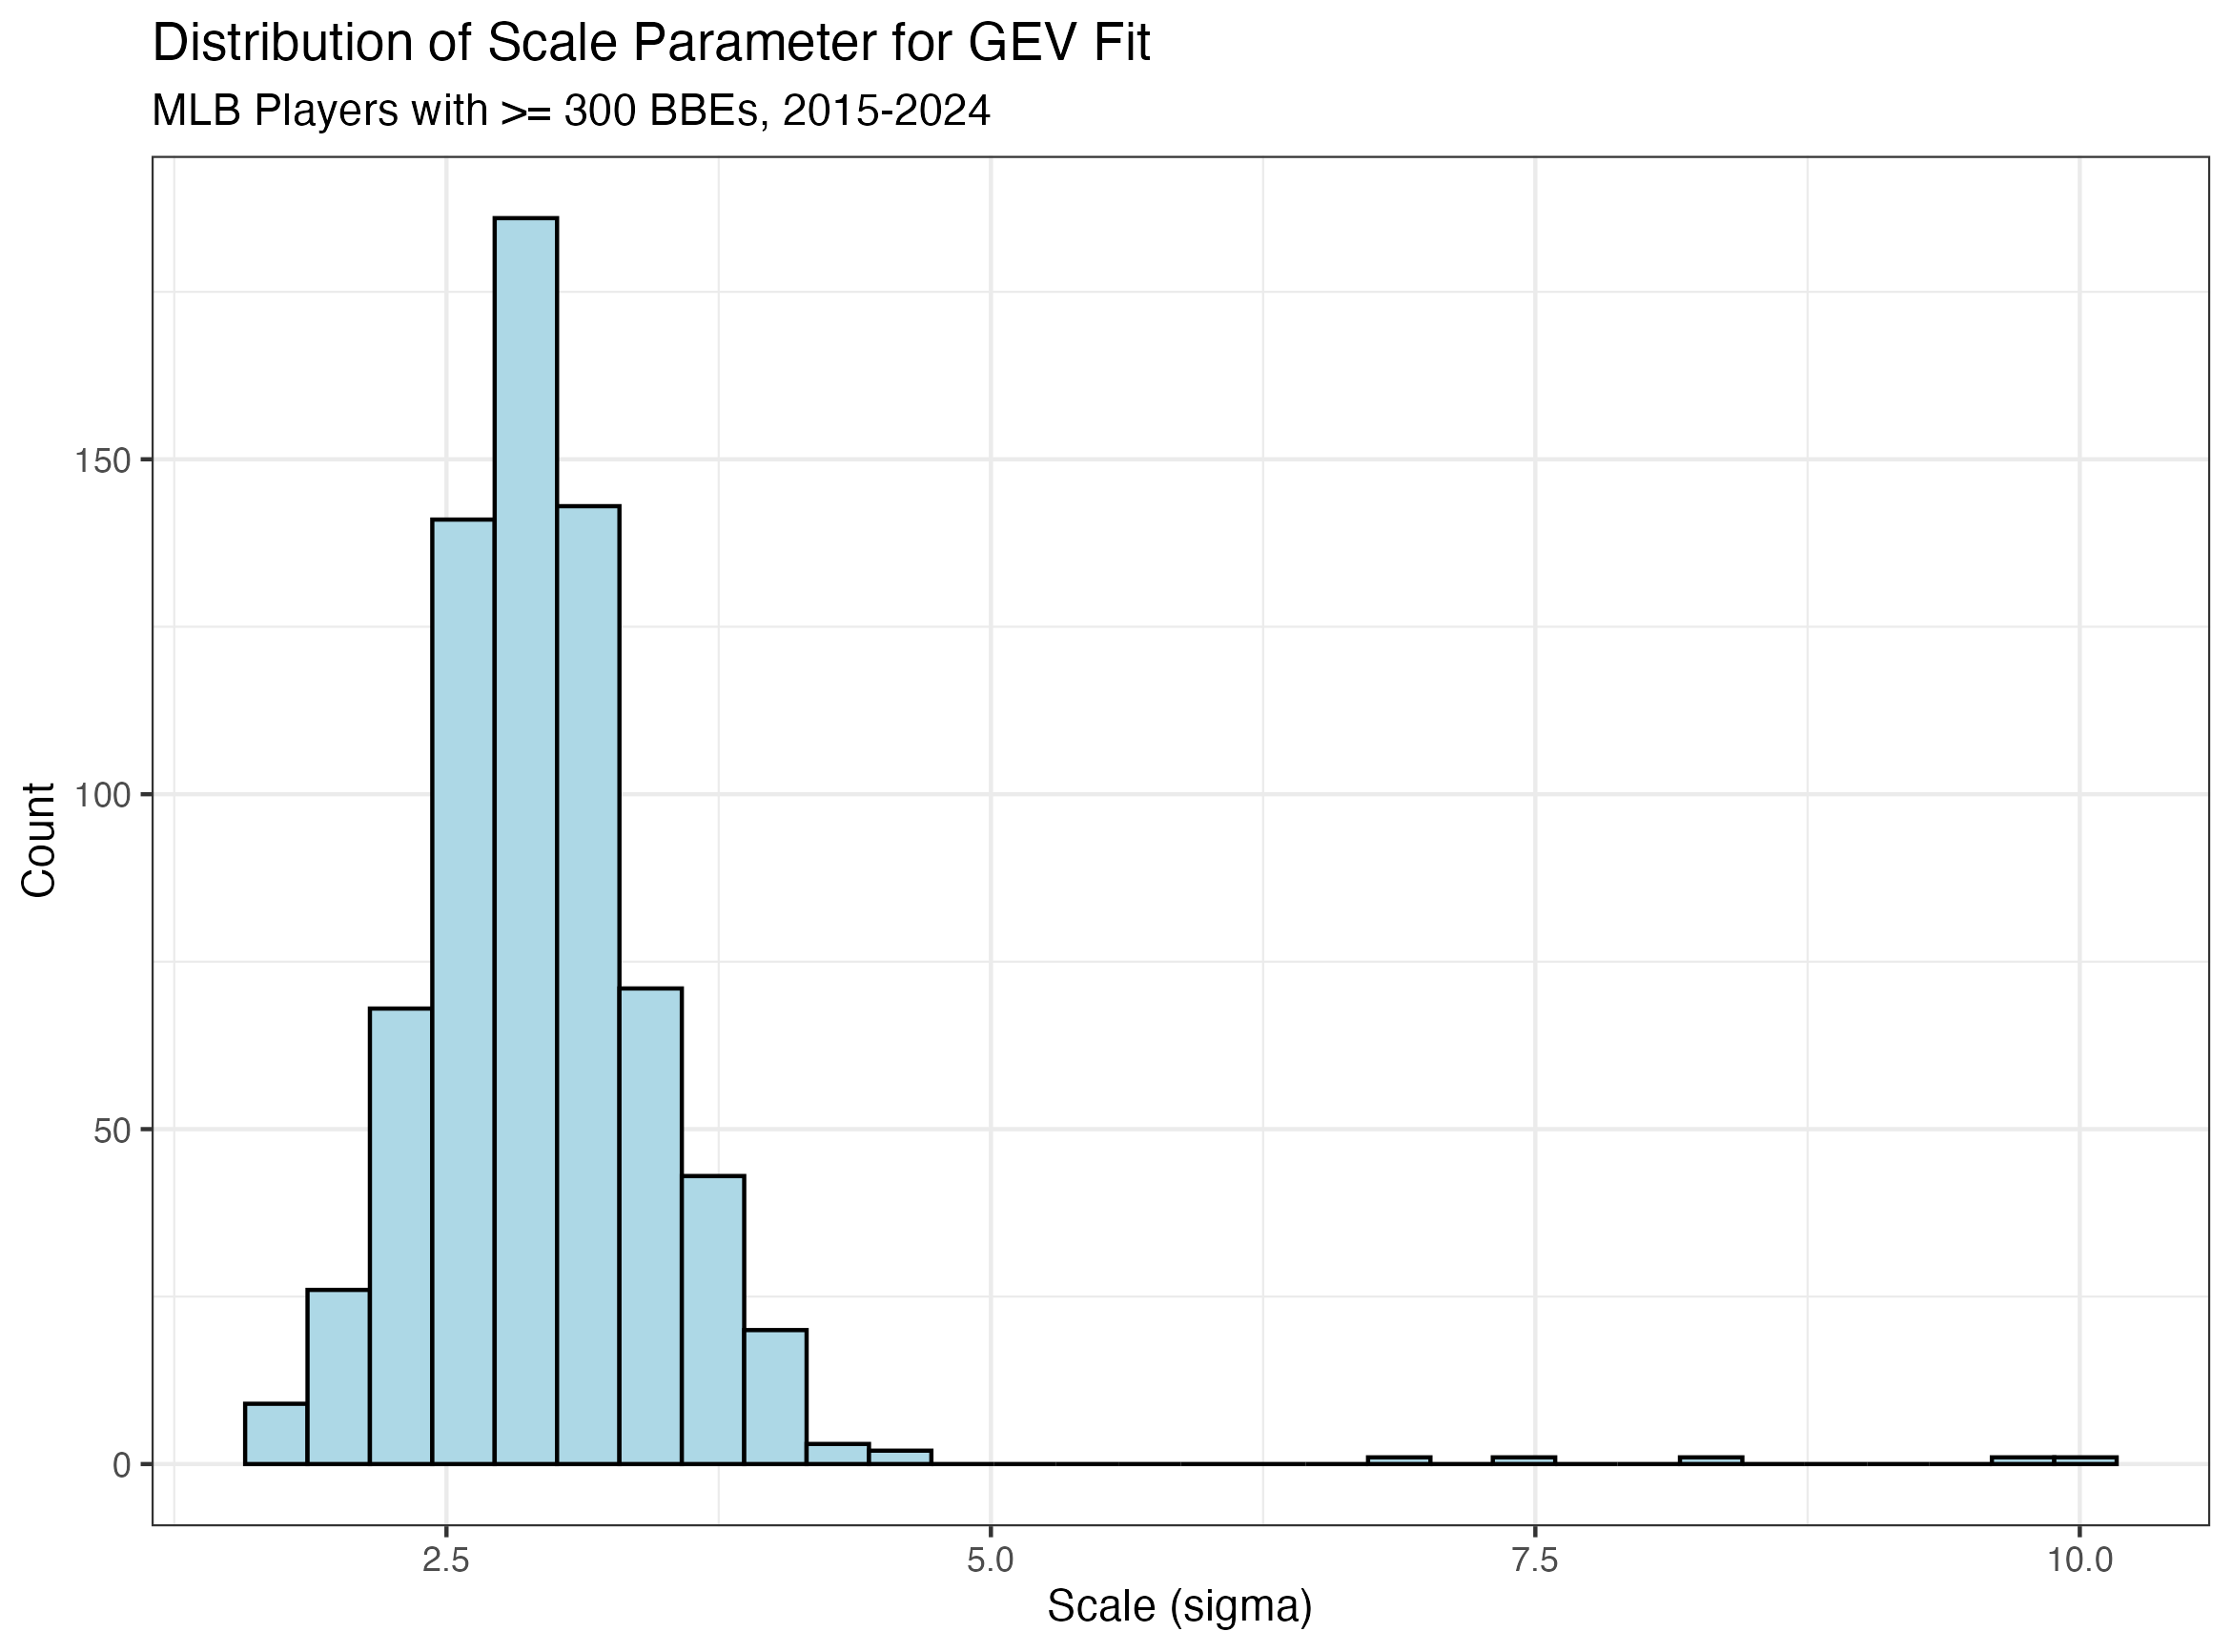
\includegraphics[width=0.49\linewidth]{plots/scale.png}
    \end{figure}
    \begin{figure}
        \centering
        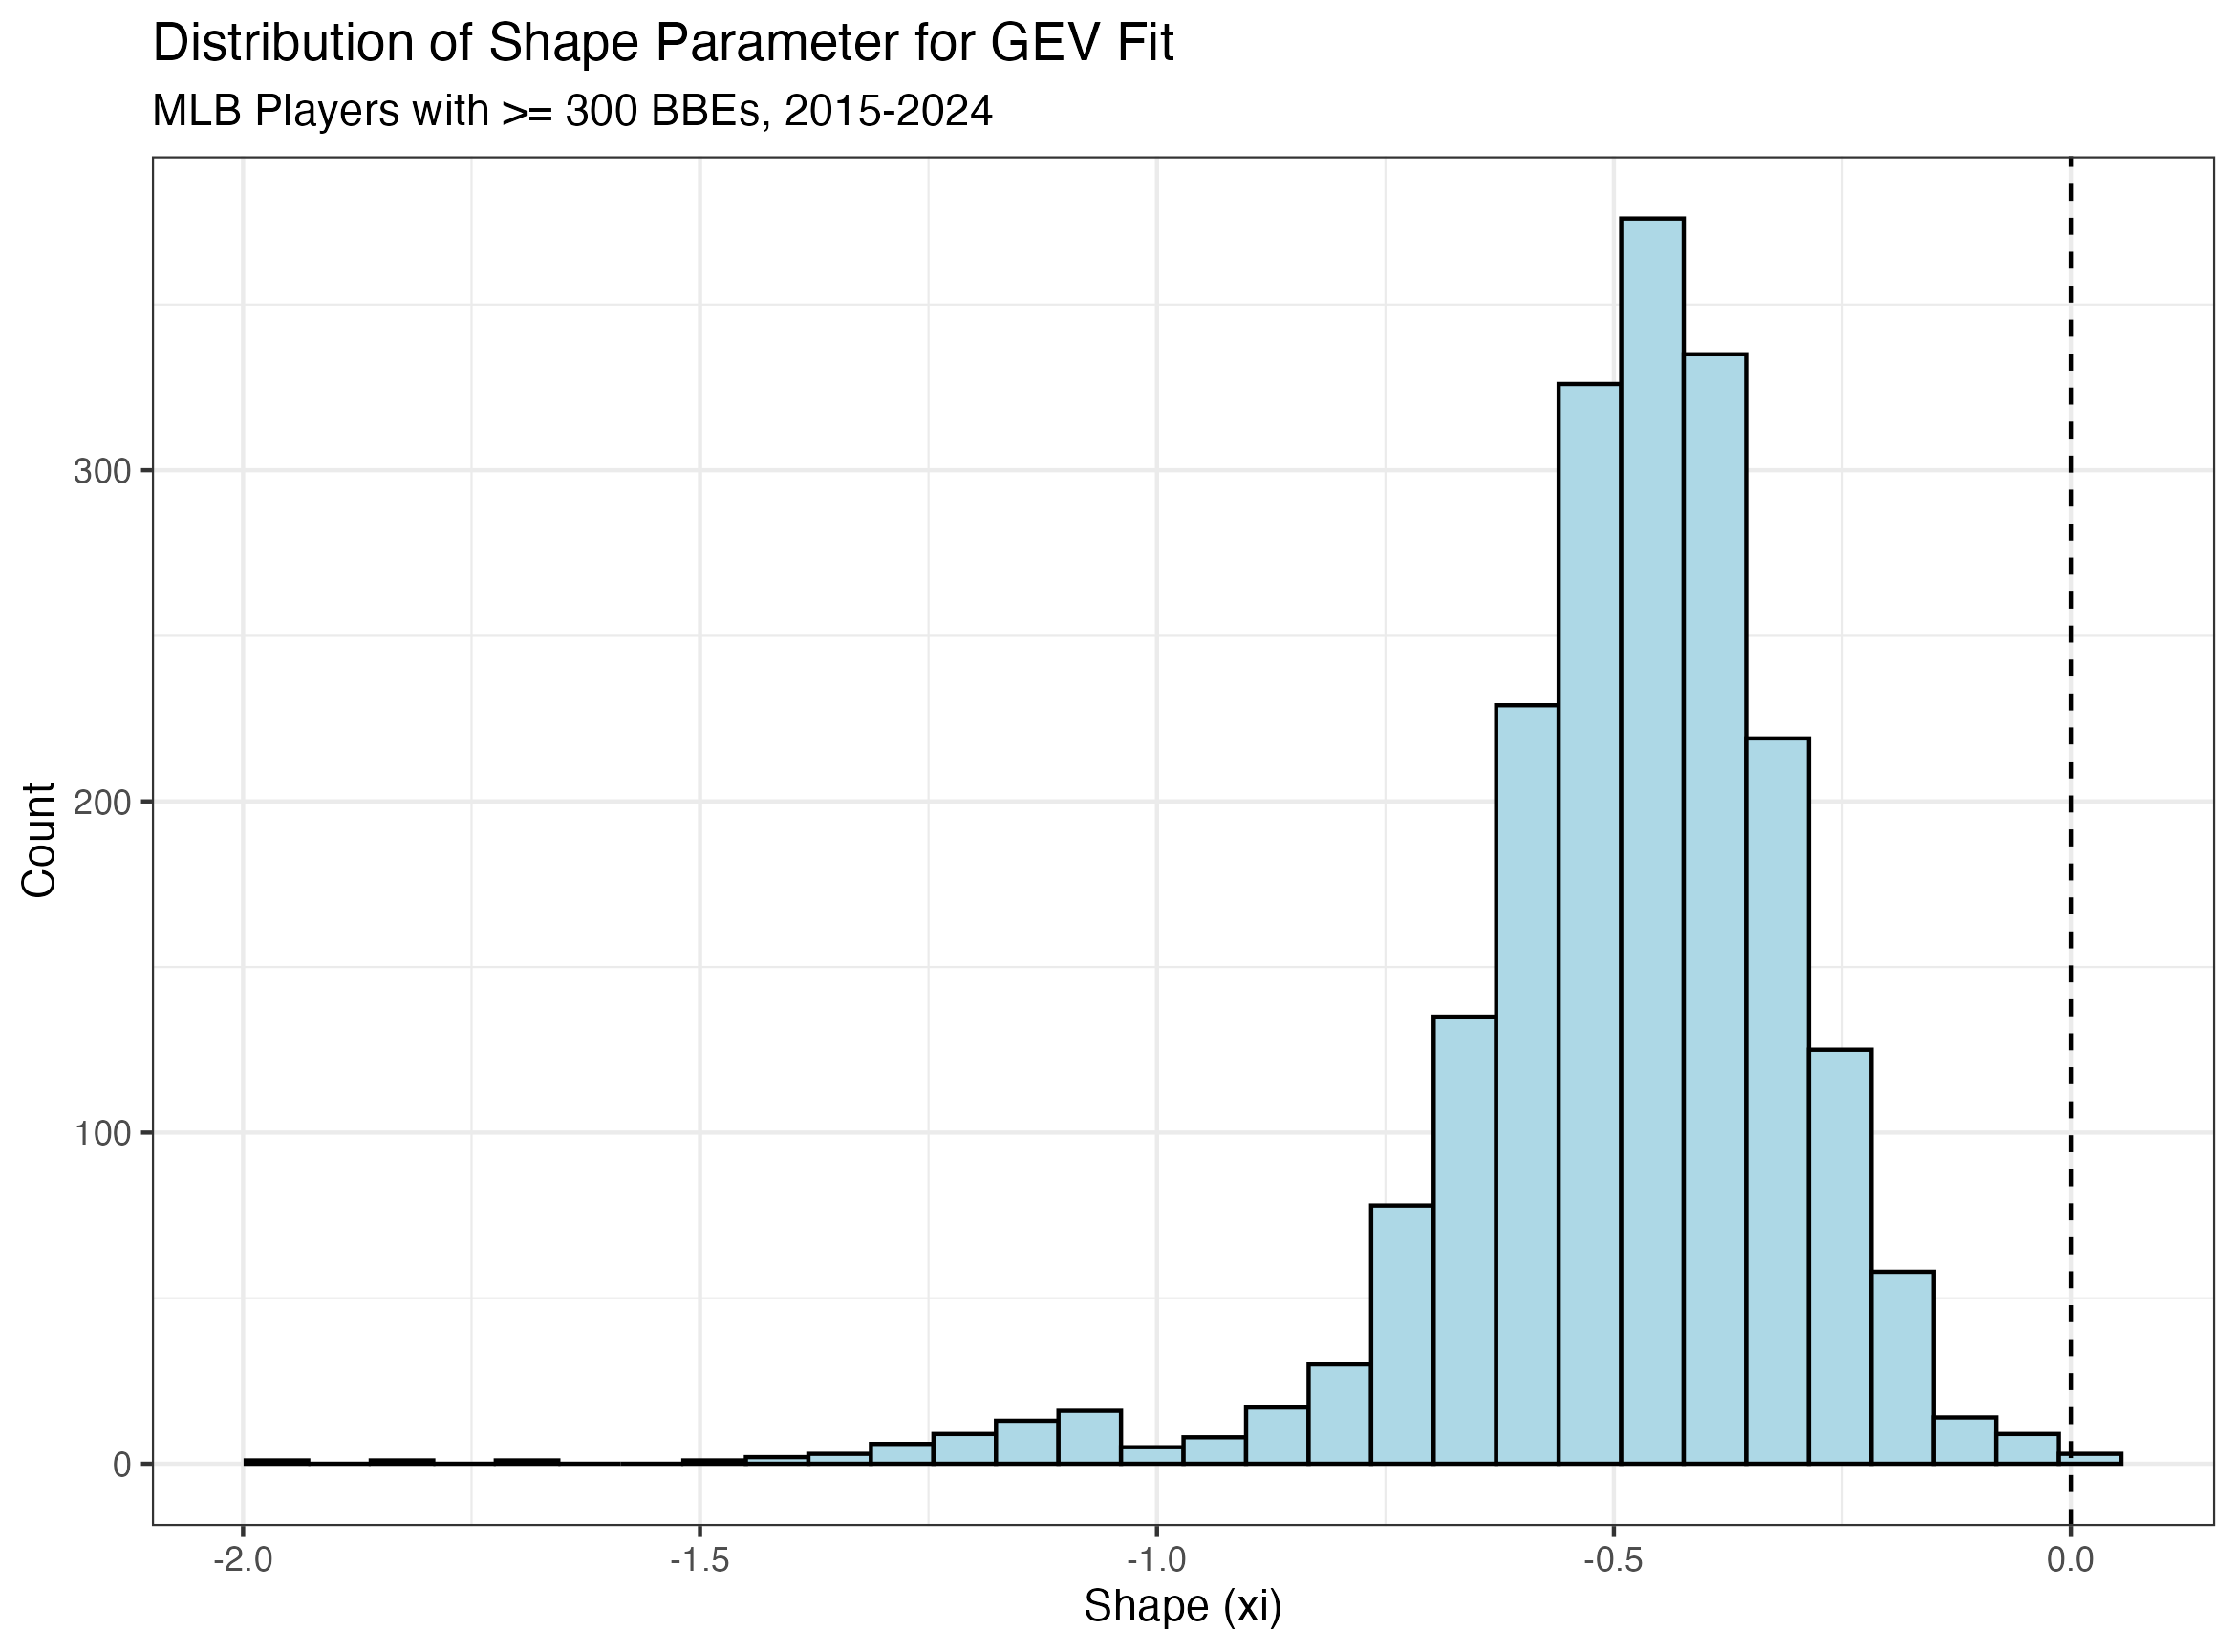
\includegraphics[width=0.85\linewidth]{plots/shape.png}
    \end{figure}
\end{frame}

\begin{frame}{Assessing Model Fit}
    For each model, we can evaluate GEV CDF at each block maximum to transform to standard uniform.
    \begin{figure}
        \centering
        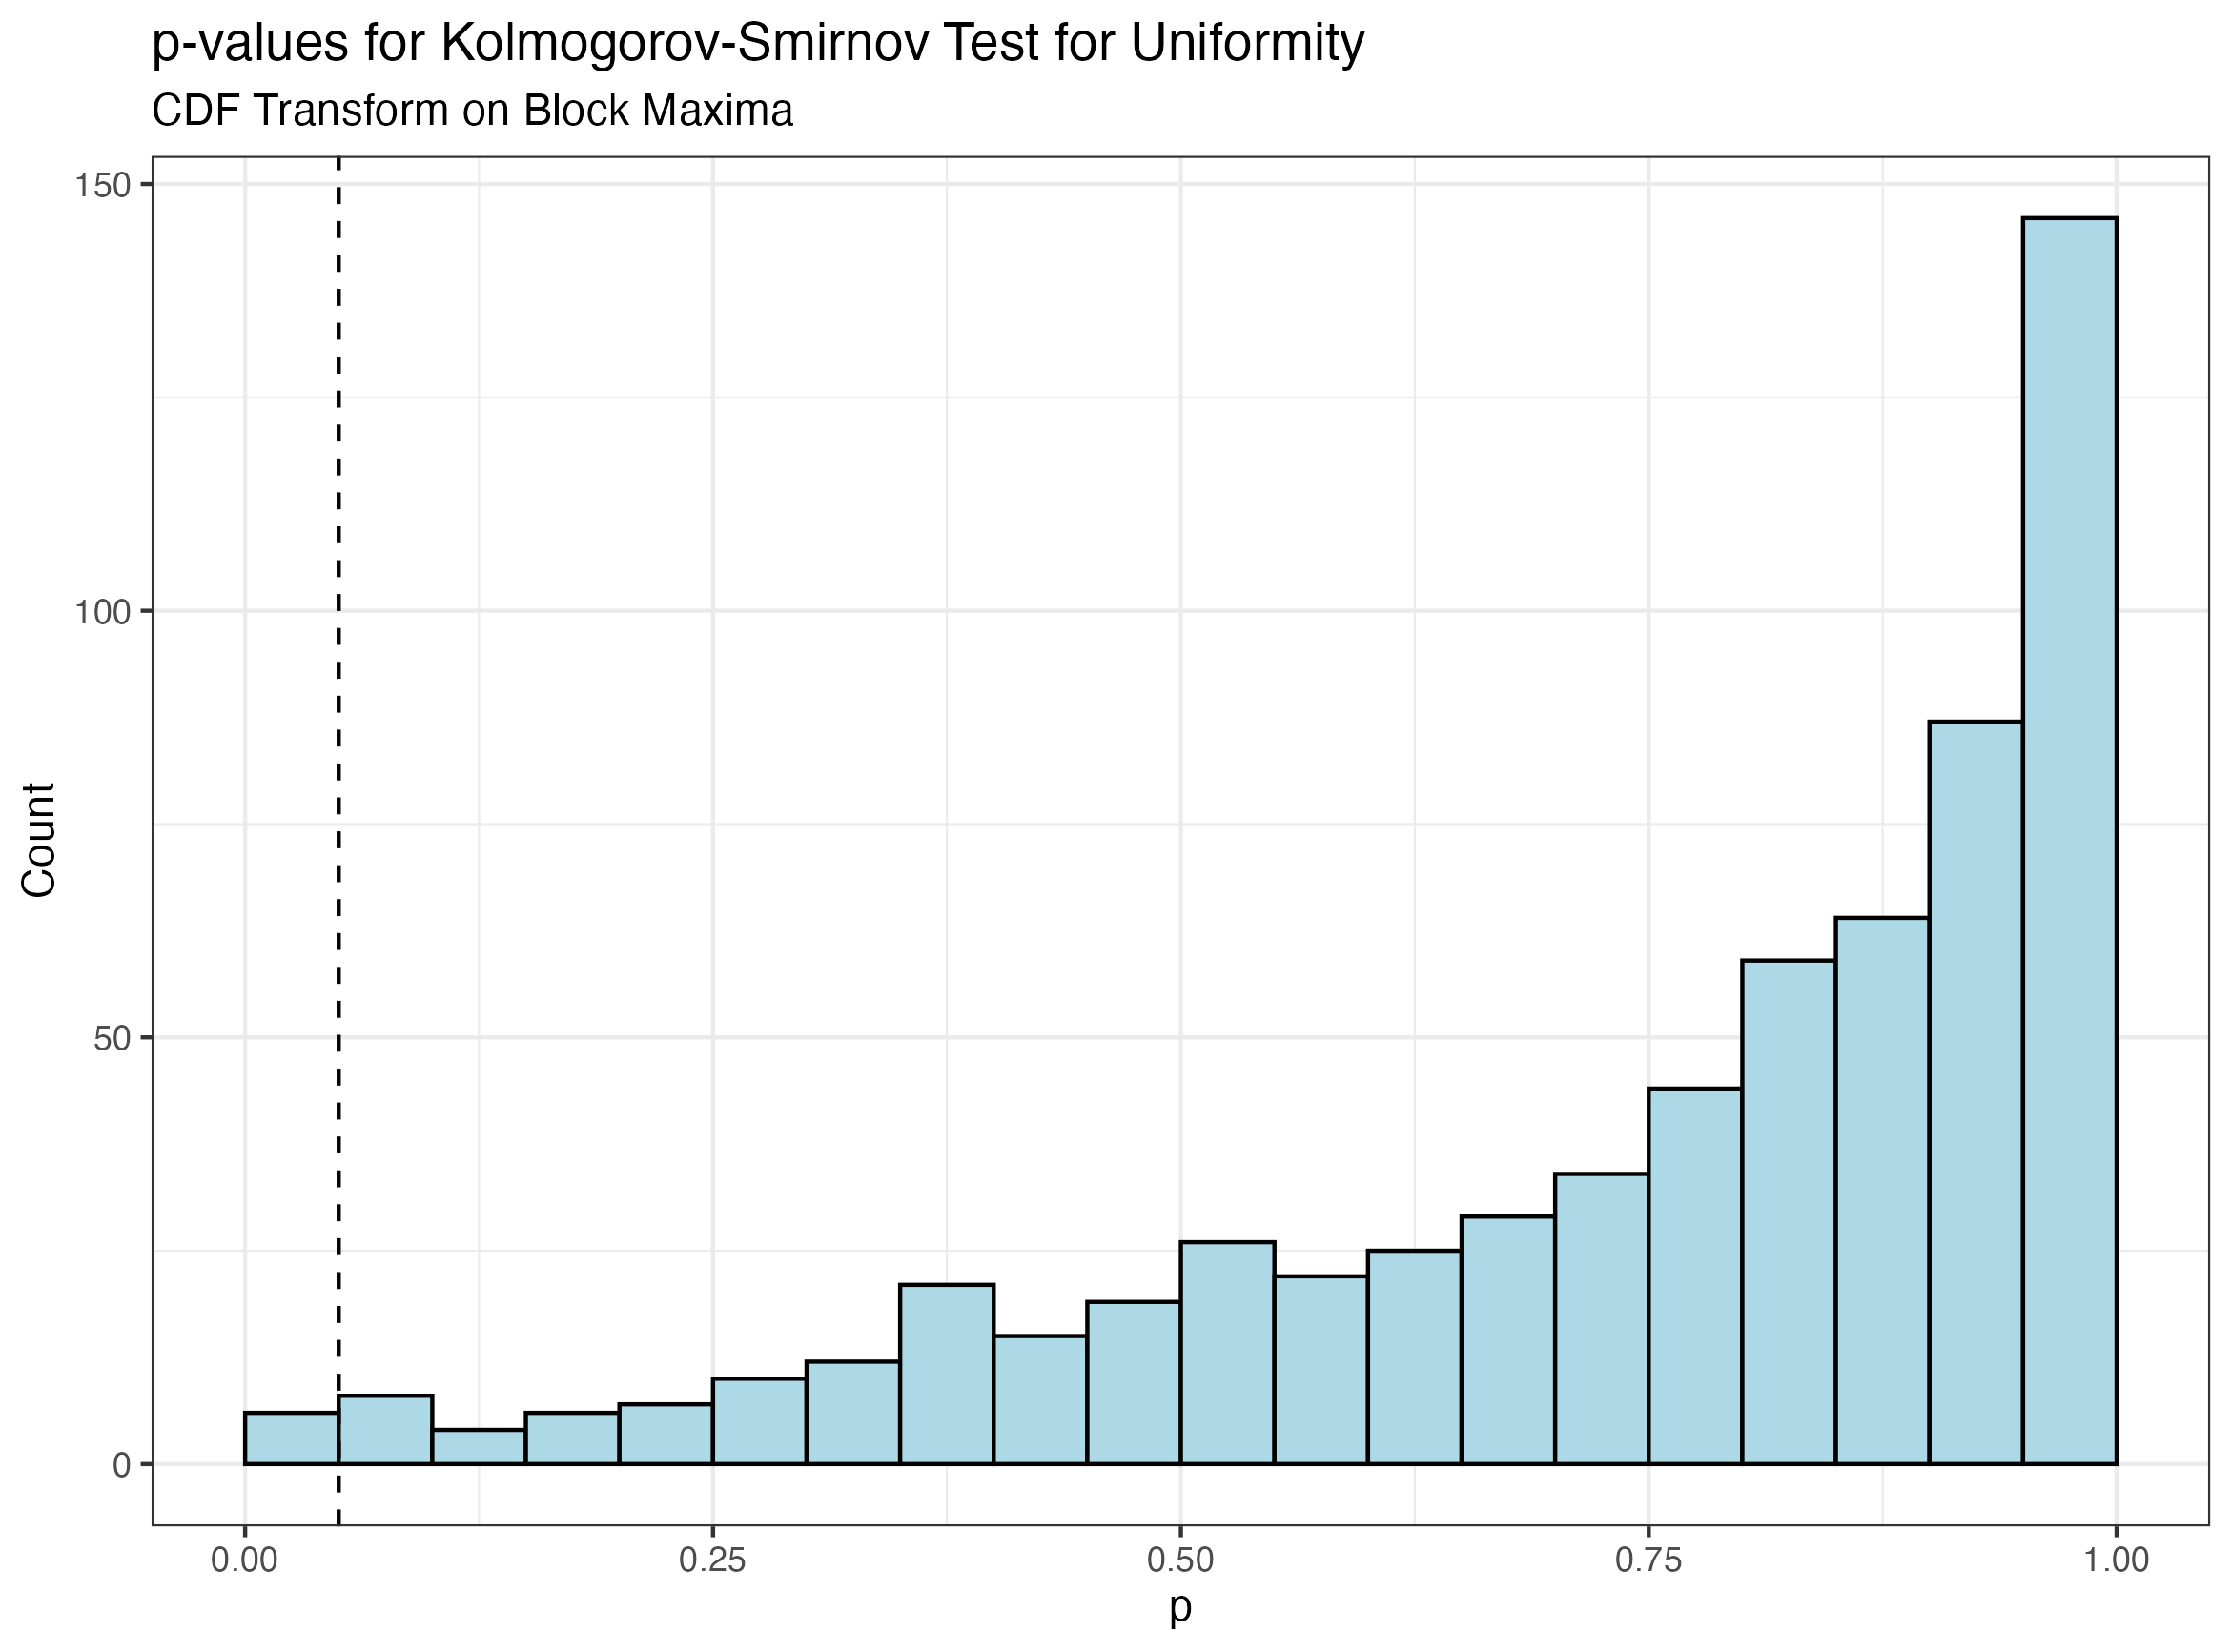
\includegraphics[width=0.85\linewidth]{plots/kstest.png}
    \end{figure}
\end{frame}

\section{Applications}
\begin{frame}{Correlation with Results}
    Use GEV fit to calculate a $5$-block (i.e. 50 BIP) return level for each player:
    \begin{figure}
        \centering
        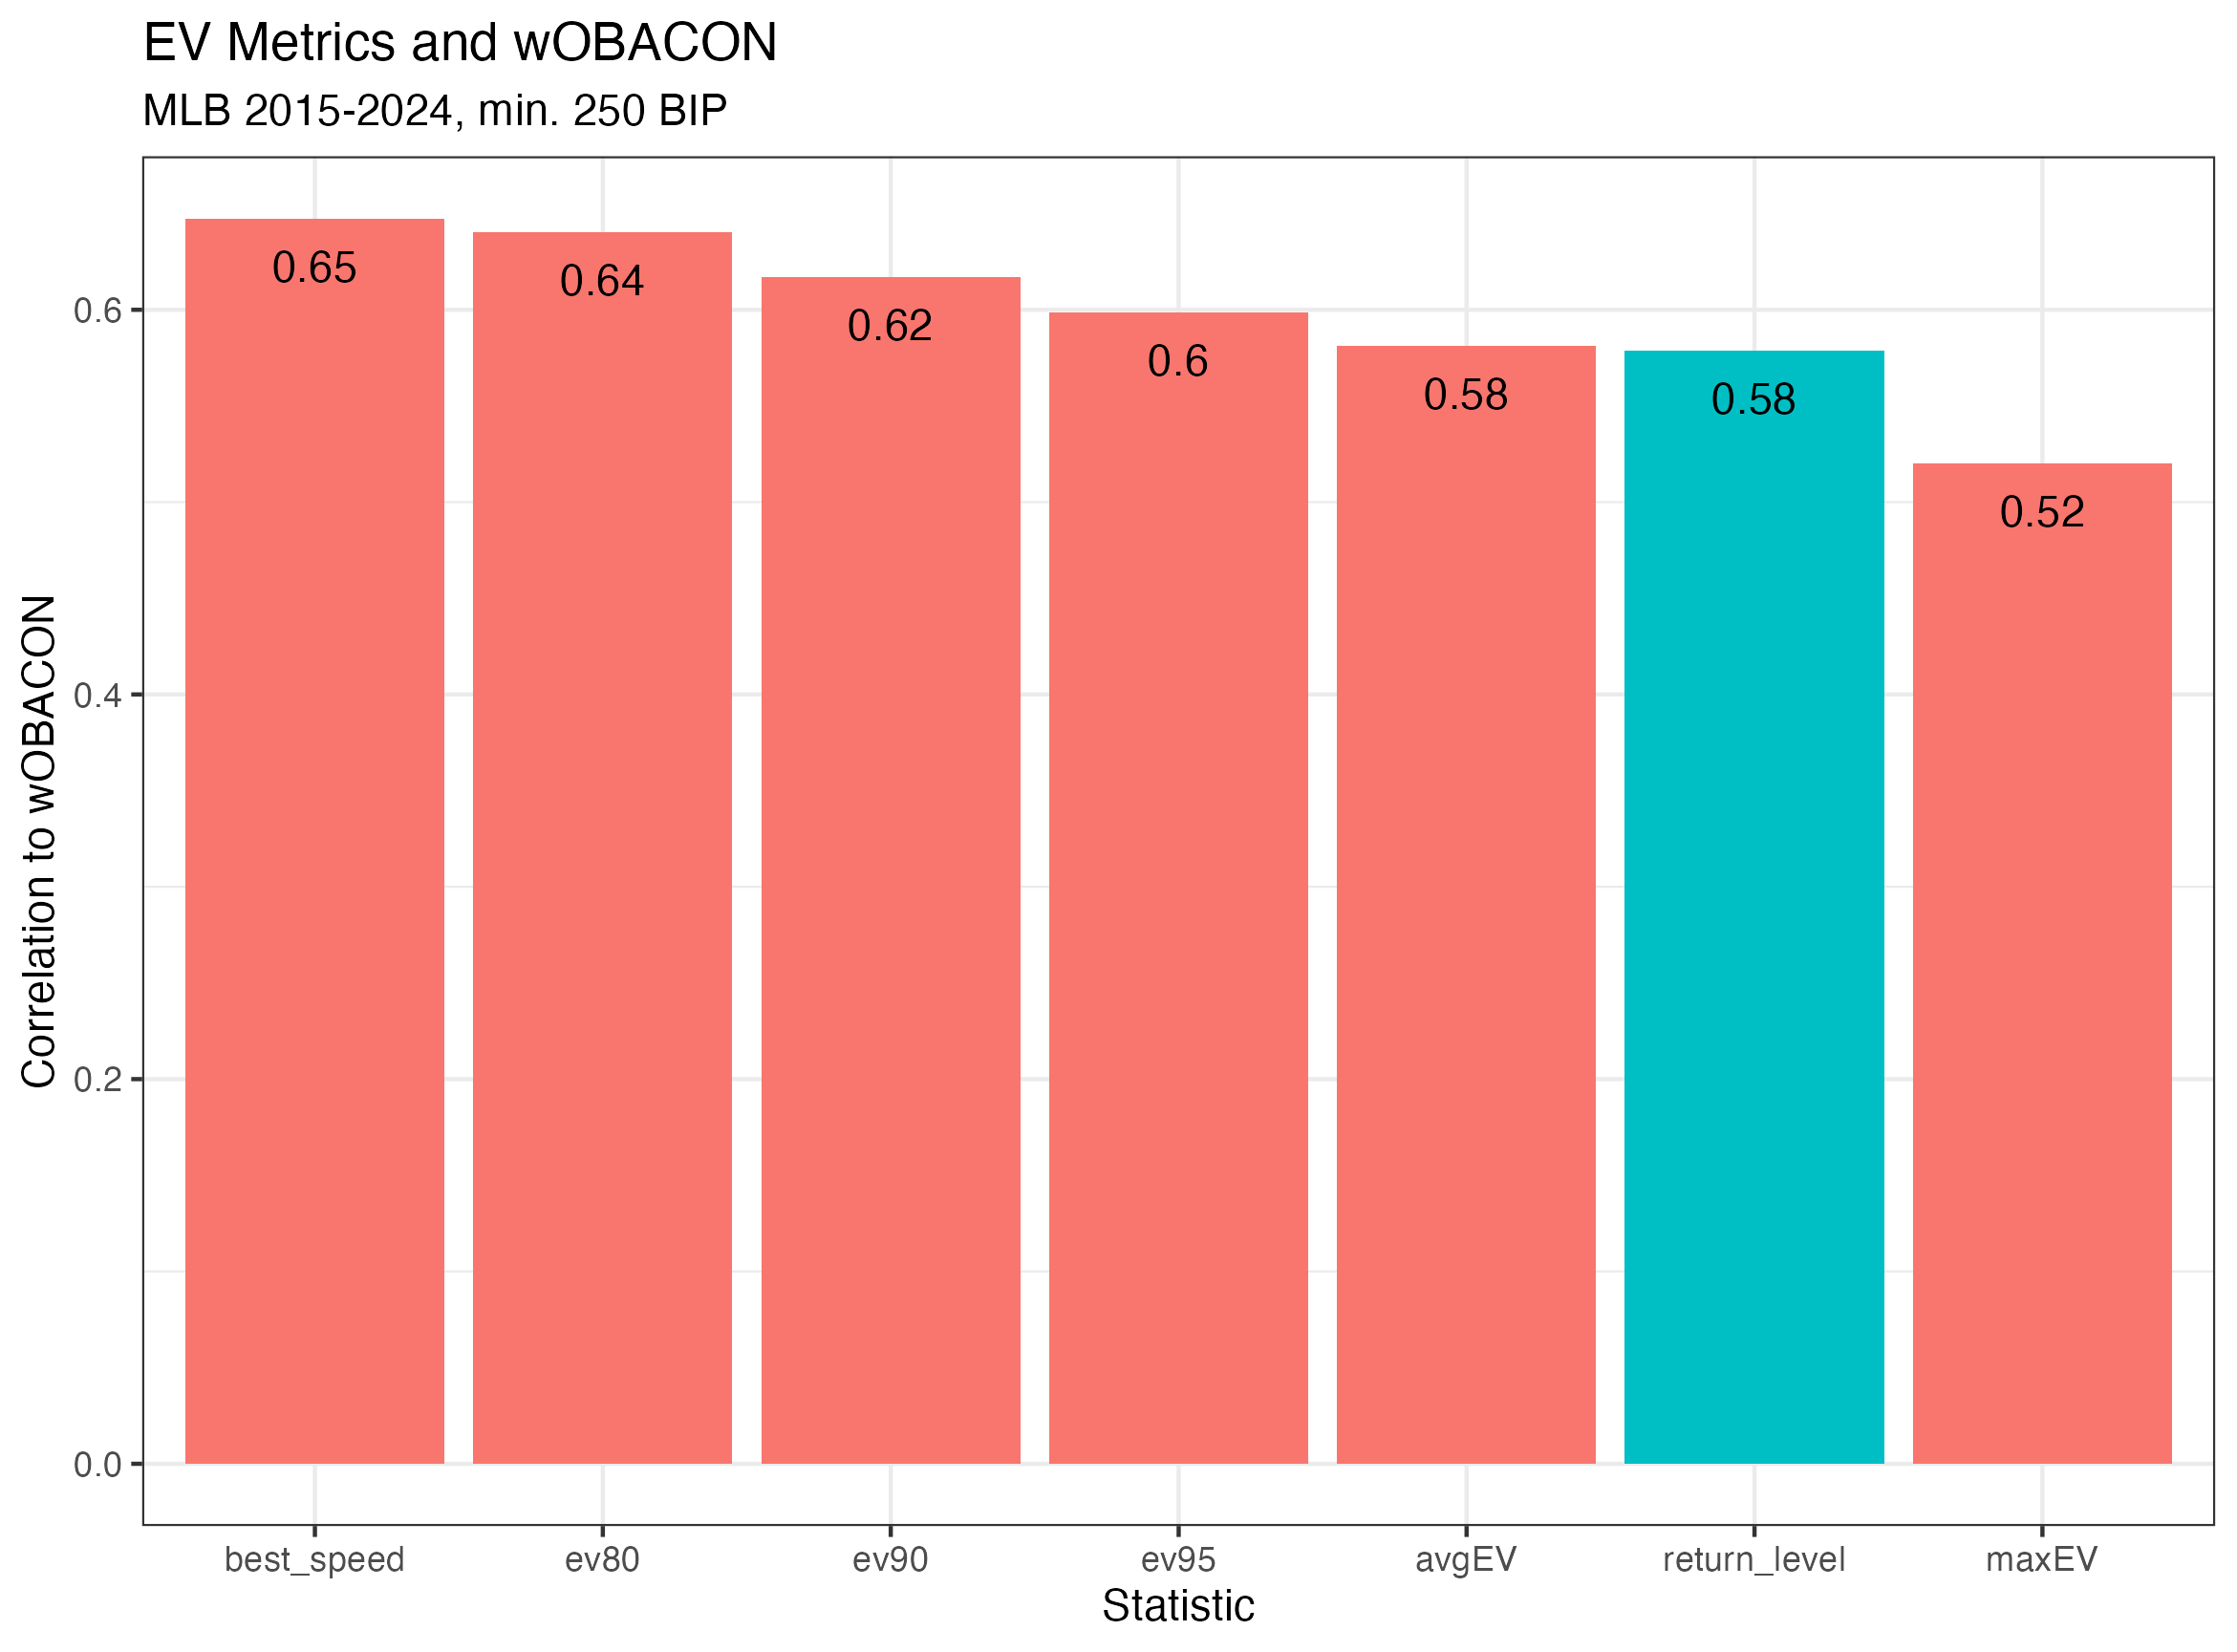
\includegraphics[width=0.85\linewidth]{plots/woba_correlation.png}
    \end{figure}
\end{frame}

\begin{frame}{Predictive Value}
    \begin{figure}
        \centering
        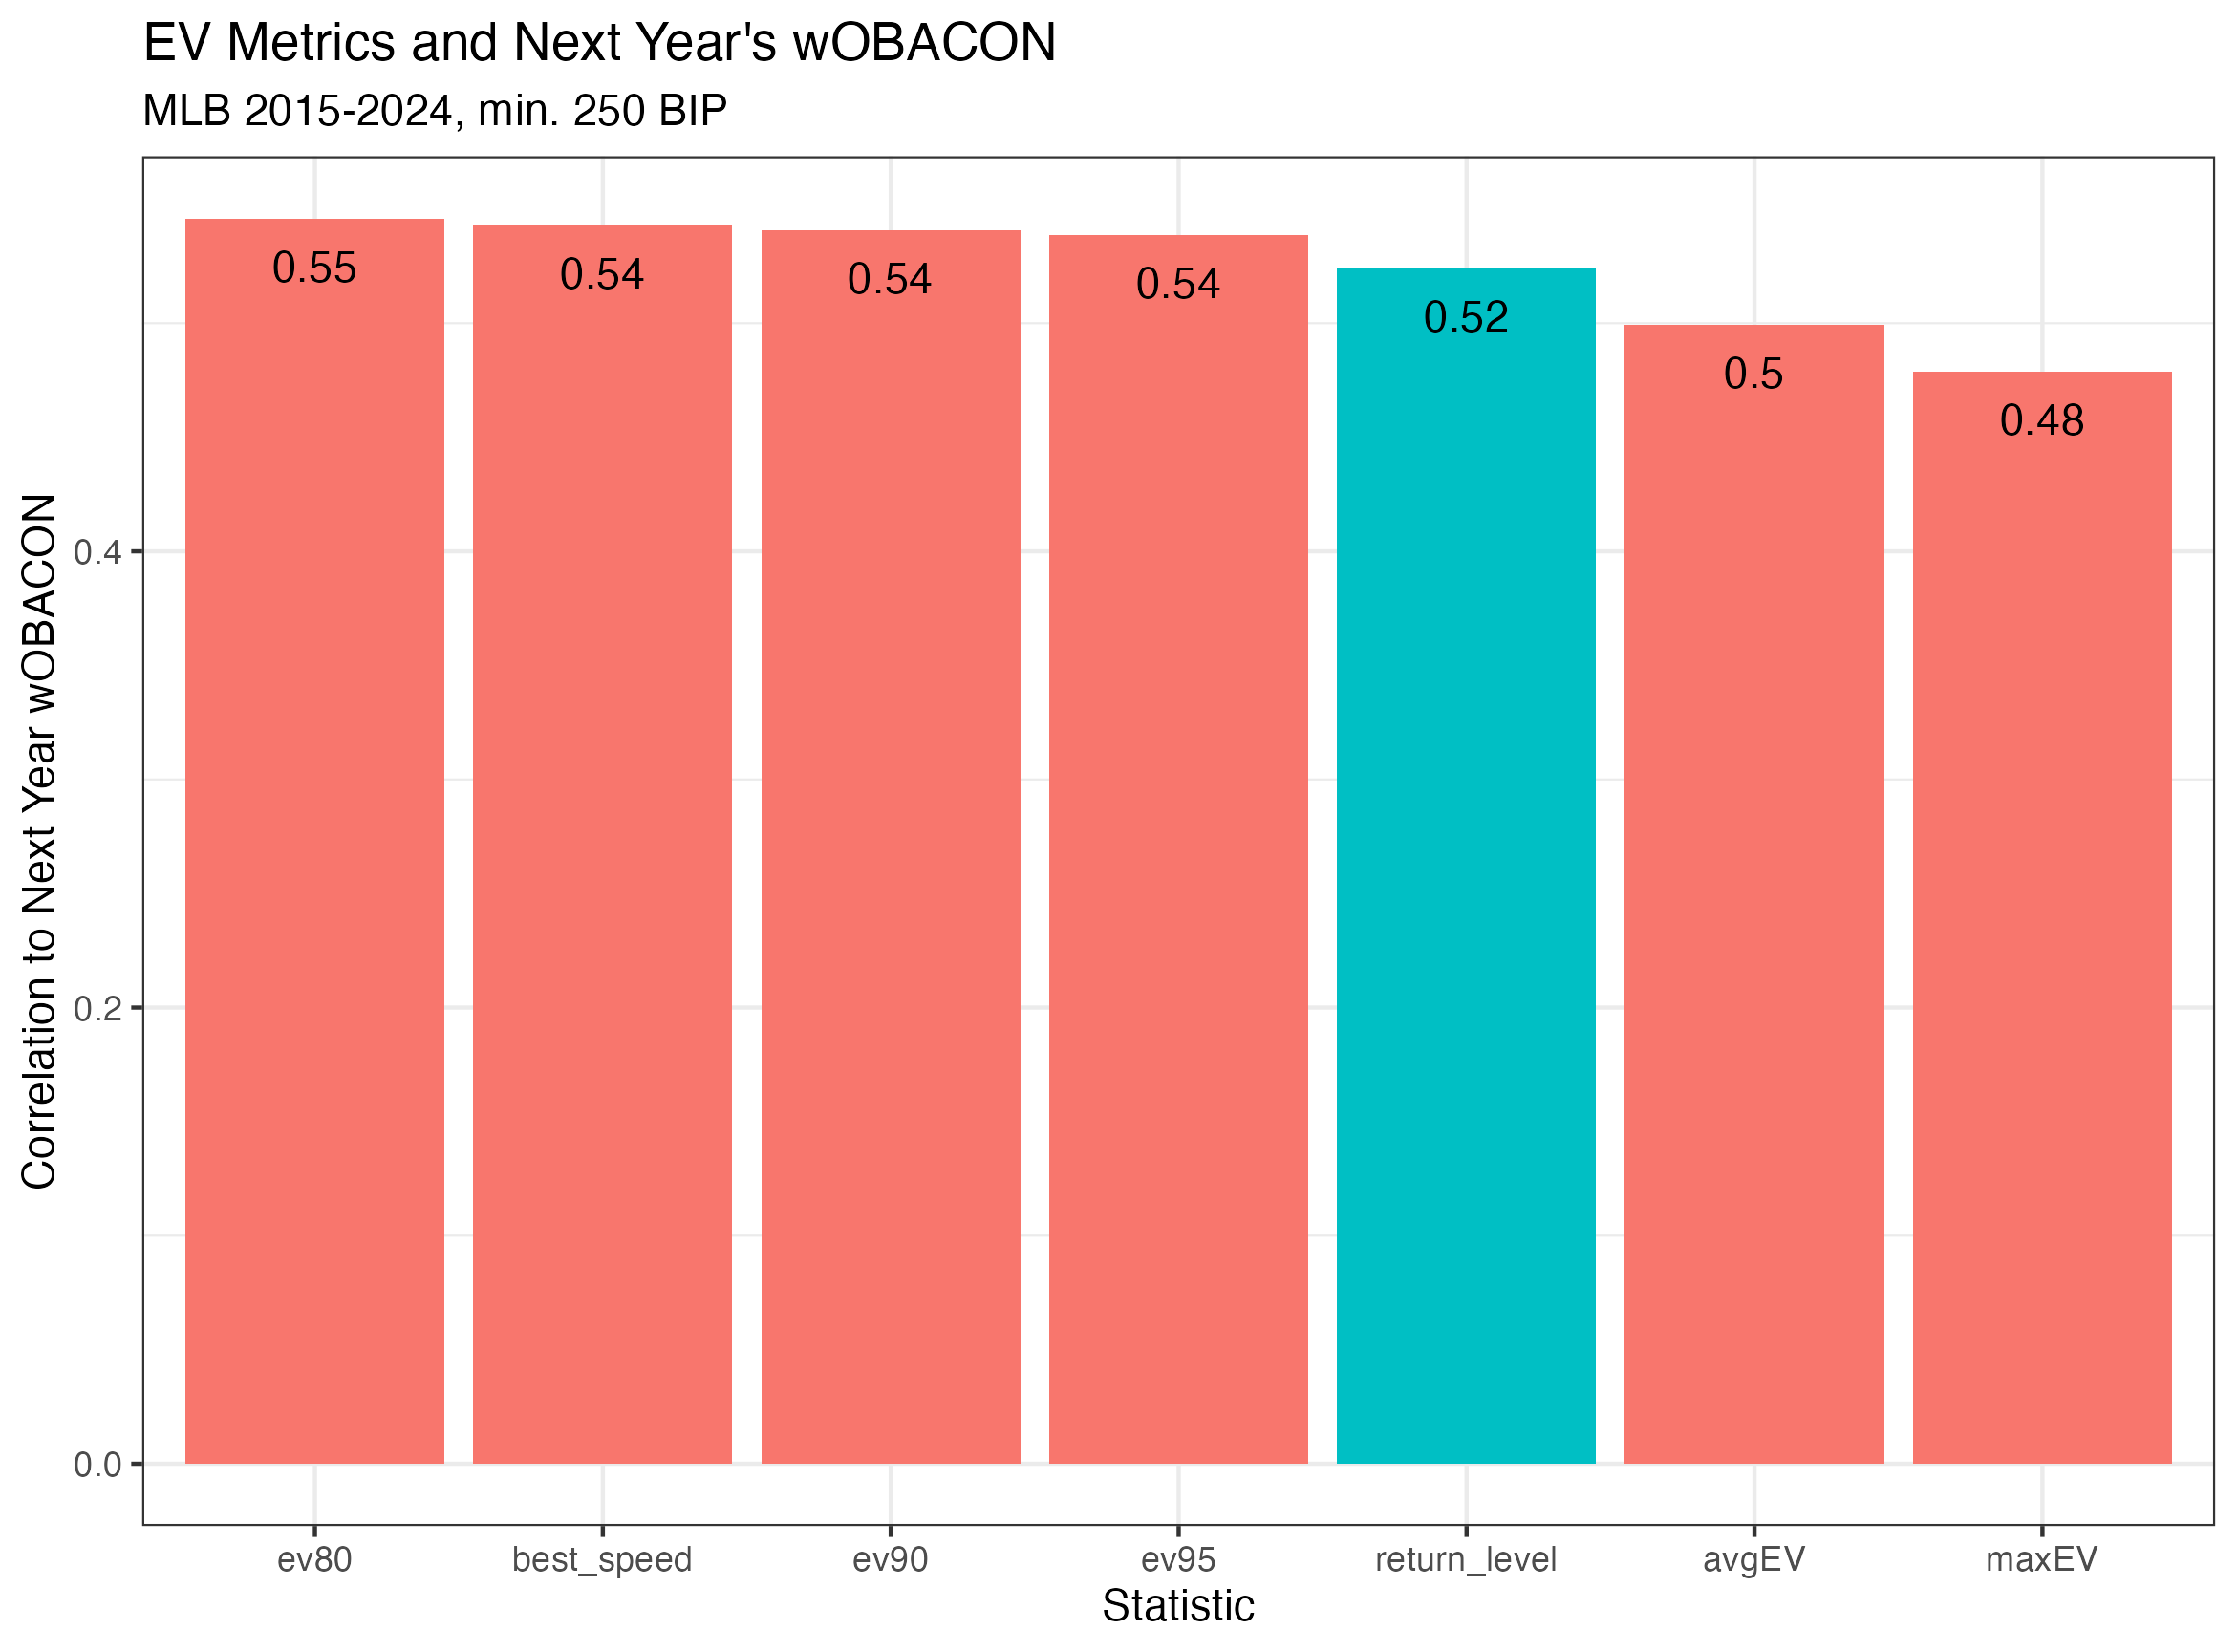
\includegraphics[width=0.85\linewidth]{plots/woba_next_correlation.png}
    \end{figure}
\end{frame}

\begin{frame}{Predicting maxEV}
    \begin{figure}
        \centering
        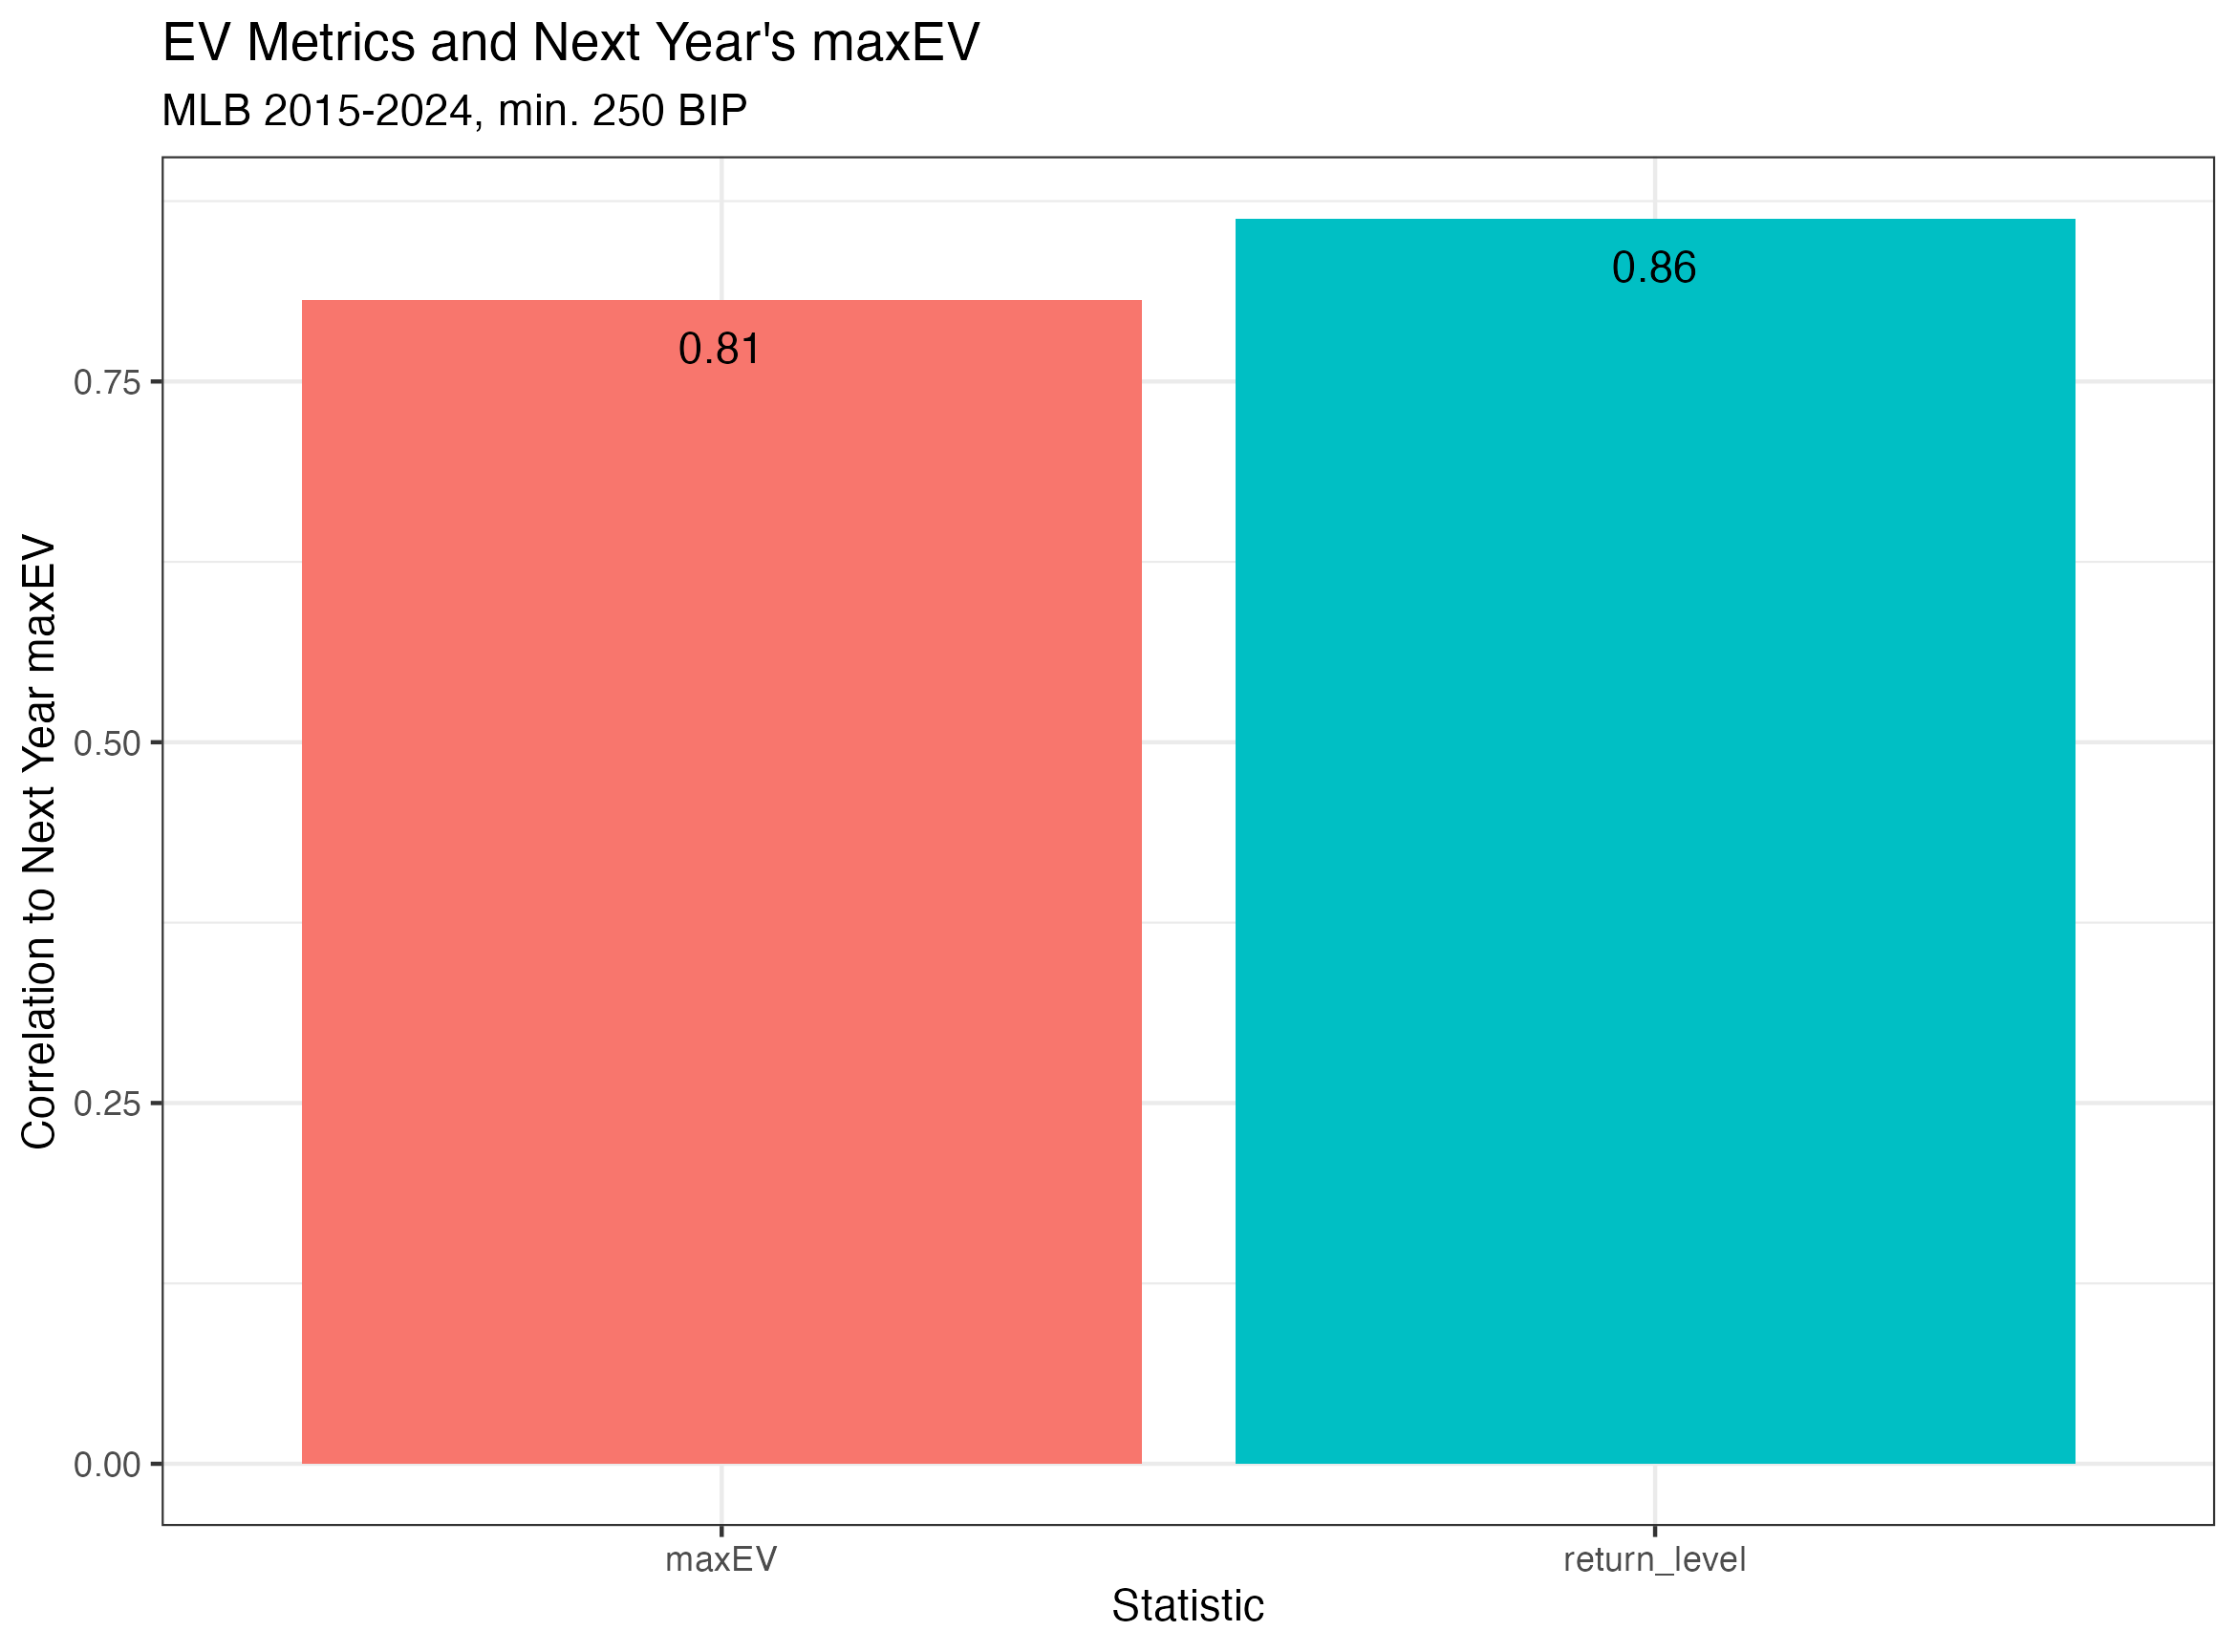
\includegraphics[width=0.85\linewidth]{plots/maxev_next_correlation.png}
    \end{figure}
\end{frame}

\begin{frame}[allowframebreaks]{Variability}
    \begin{figure}
        \centering
        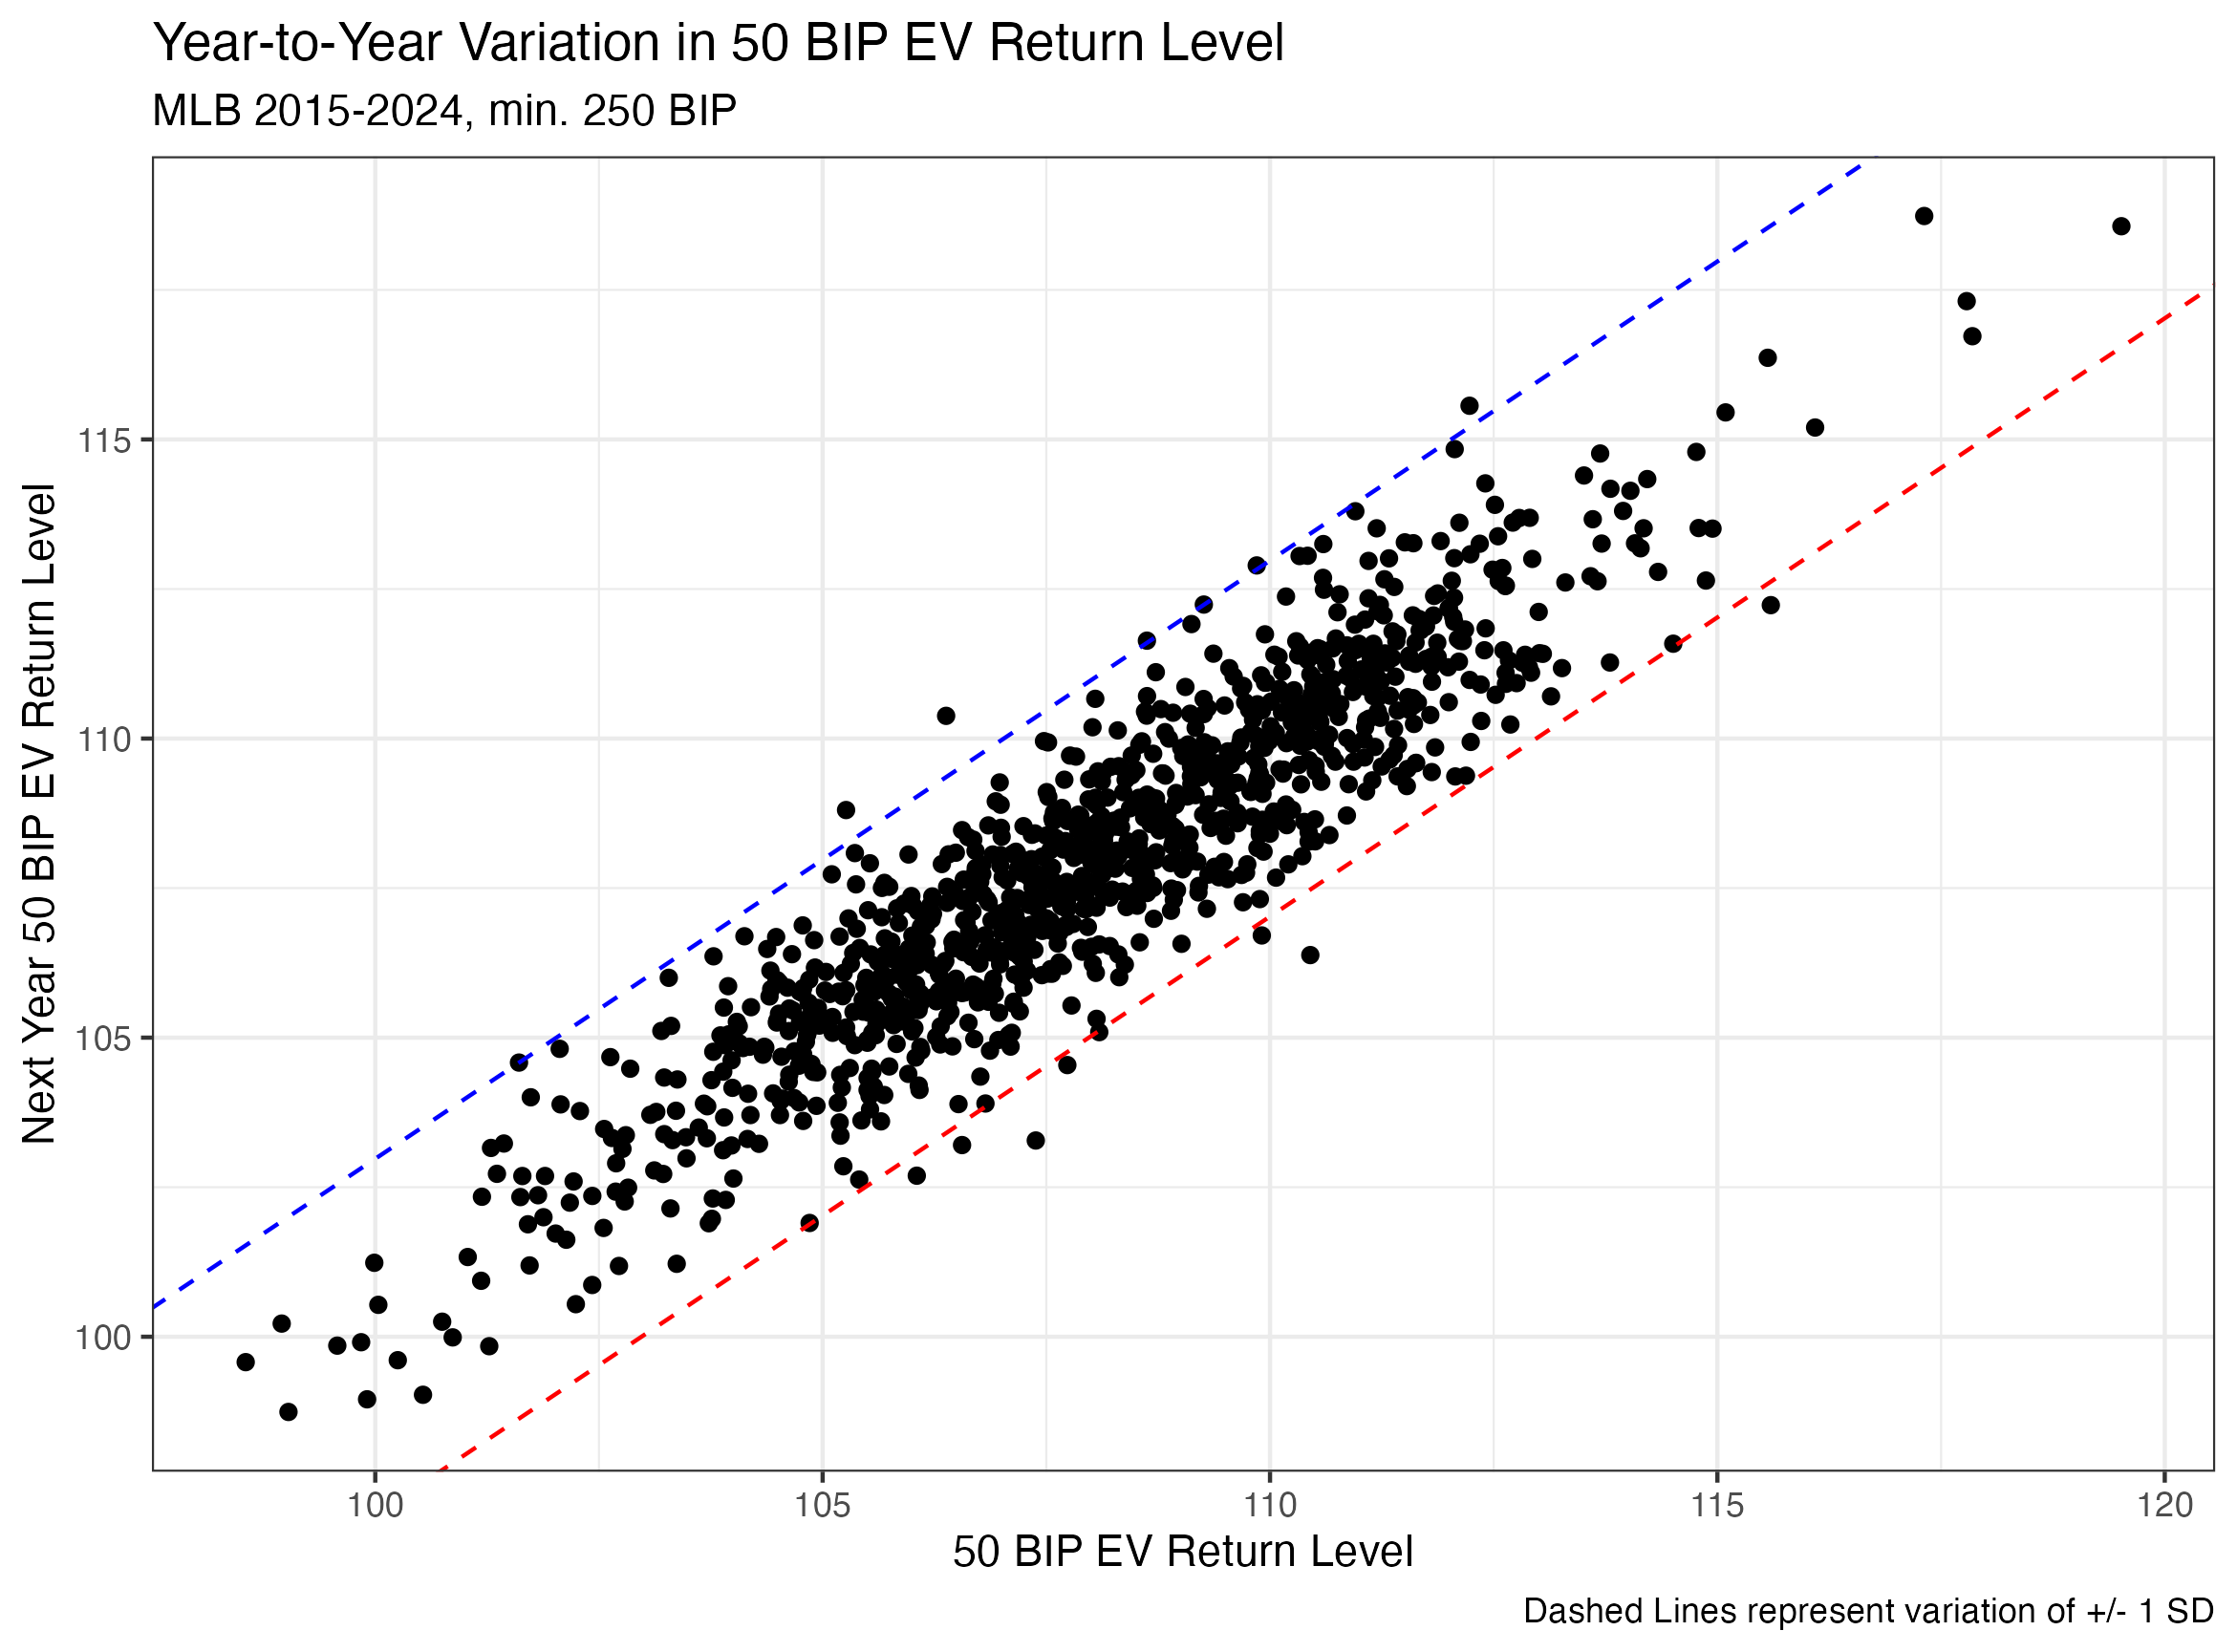
\includegraphics[width=0.85\linewidth]{plots/return_level_stability.png}
    \end{figure}
    \begin{figure}
        \centering
        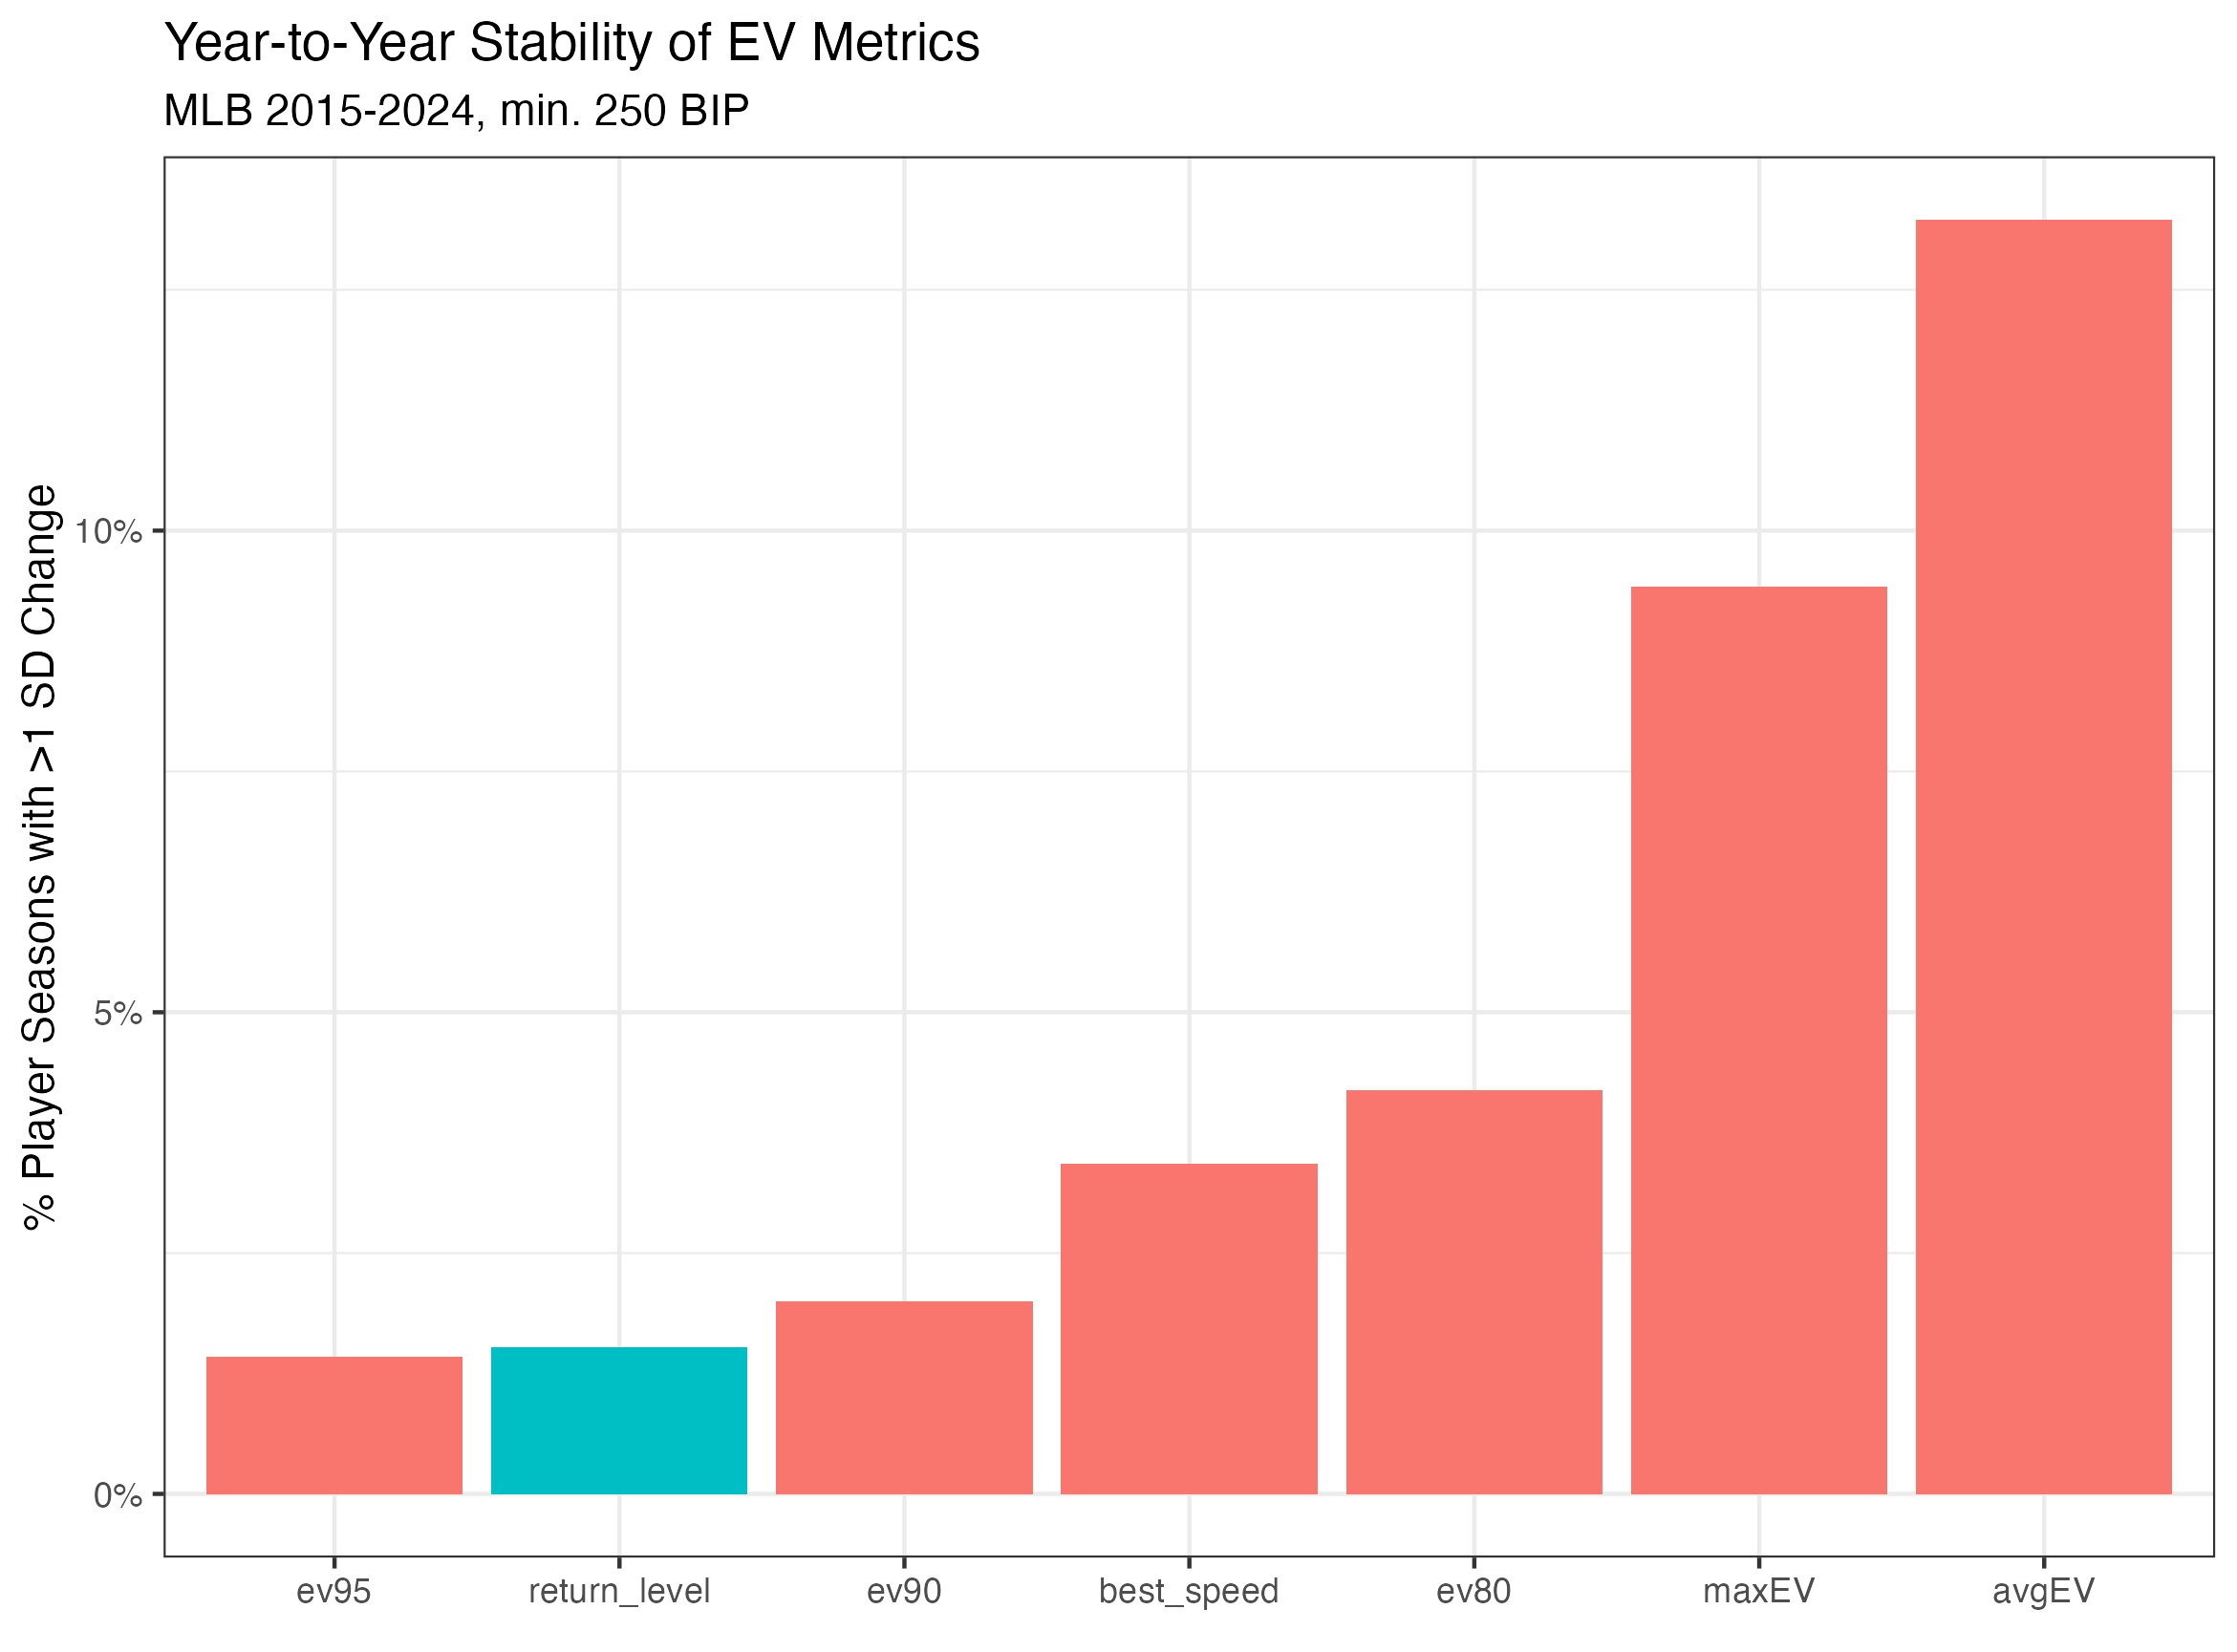
\includegraphics[width=0.85\linewidth]{plots/stability.png}
    \end{figure}
\end{frame}

\begin{frame}[allowframebreaks]
    \printbibliography
\end{frame}
\end{document}